\section{Detailed Results}
\label{sec:benchs-pres}

In the following section we show the results of the competition from the benchmark's perspective. 
For a given benchmark we would like to know: how many solvers solved it, what is the min and max time to solve,  what are the min and max size of the expressions produced, which solver solved the benchmark the fastest, and which solver produced the smallest expression.



We represents the results per benchmark in groups organized per tracks and categories. For instance, Fig.~\ref{fig:prog-rep-icfp} at the top presents details of the program repair benchmarks. The black bars show the range of the time to solve among the different solvers in pseudo logarithmic scale (as indicated on the upper part of the y-axis). Inspect for instance benchmark \texttt{t\_2.sl}. The black bar indicates that the fastest solver to solve it used less than 1 second, and the slowest used between 100 to 300 seconds. 
The black number above the black bar indicates the exact number of seconds (floor-rounded to the nearest second) it took the slowest solver to solve a benchmark (and $\infty$ if at least one solver exceeded the time bound). Thus, we can see that the slowest solver to solve \texttt{t\_2.sl} took 141 seconds to solve it. The white number at the lower part of the bar indicates the time of the fastest solver to solve that benchmark. Thus, we can see that the fastest solver to solve \texttt{t\_2.sl} required less than 1 second to do so. The colored squares/rectangles next to the lower part of the black bar, indicate which solvers were the fastest to solve that benchmark (according to the solvers' legend at the top). Here, \emph{fastest} means in the same logarithmic scale as the absolute fastest solver. For instance, we can see that \euphony\ and \eusolvernew\ were the fastest to solve \texttt{t\_2.sl}, solving it in less than a second
and that among the 2 solvers that solved \texttt{t\_3.sl} only \eusolvernew\ solved it in less than 1 seconds. 

Similarly, the gray bars indicate the range of expression sizes in pseudo logarithmic scales (as indicated on the lower part of the y-axis), where the size of an expression is determined by the number of nodes in its parse tree.
The black number at the bottom of the gray bar indicates the exact size expression of the largest solution (or $\infty$ if it exceeded 1000), and the white number at the top of the gray bar indicates the exact size expression of the smallest solution (when the smallest and largest size of expressions are in the same logarithmic bucket (as is the case in \texttt{t\_2.sl}), we provide only the largest expression size, thus there is no white number on the gray bar). The colored squares/rectangles next to the upper part of the gray bar indicates which solvers (according to the legend) produced the smallest expression (where \emph{smallest} means in the same logarithmic scale as the absolute smallest expression). For instance, for \texttt{t\_20.sl} the smallest expression produced had size 3, and 2 solvers out of the 3 who solved it managed to produce an expression of size less than 10.  

Finally, at the top of the figure above each benchmark there is a number indicating the number of solvers that solved that benchmark. For instance, one solver solved \texttt{t\_14.sl}, two solvers solved \texttt{t\_12.sl}, three solvers solved \texttt{t\_2.sl}, and no solver solved \texttt{t\_6.sl}. Note that the reason \texttt{t\_6.sl} has 2 as the upper time bound, is that that is the time to terminate rather than the time to solve. Thus, all solvers aborted within less than 2 seconds, but either they did not produce a result, or they produced an incorrect result. When no solver produced a correct result, there are no colored squares/rectangles next to the lower parts of the bars, as is the case for \texttt{t\_6.sl}.


\begin{figure*}
	\noindent\makebox[\textwidth]{
		\scalebox{0.625}{
			\begin{tabular}{c}
				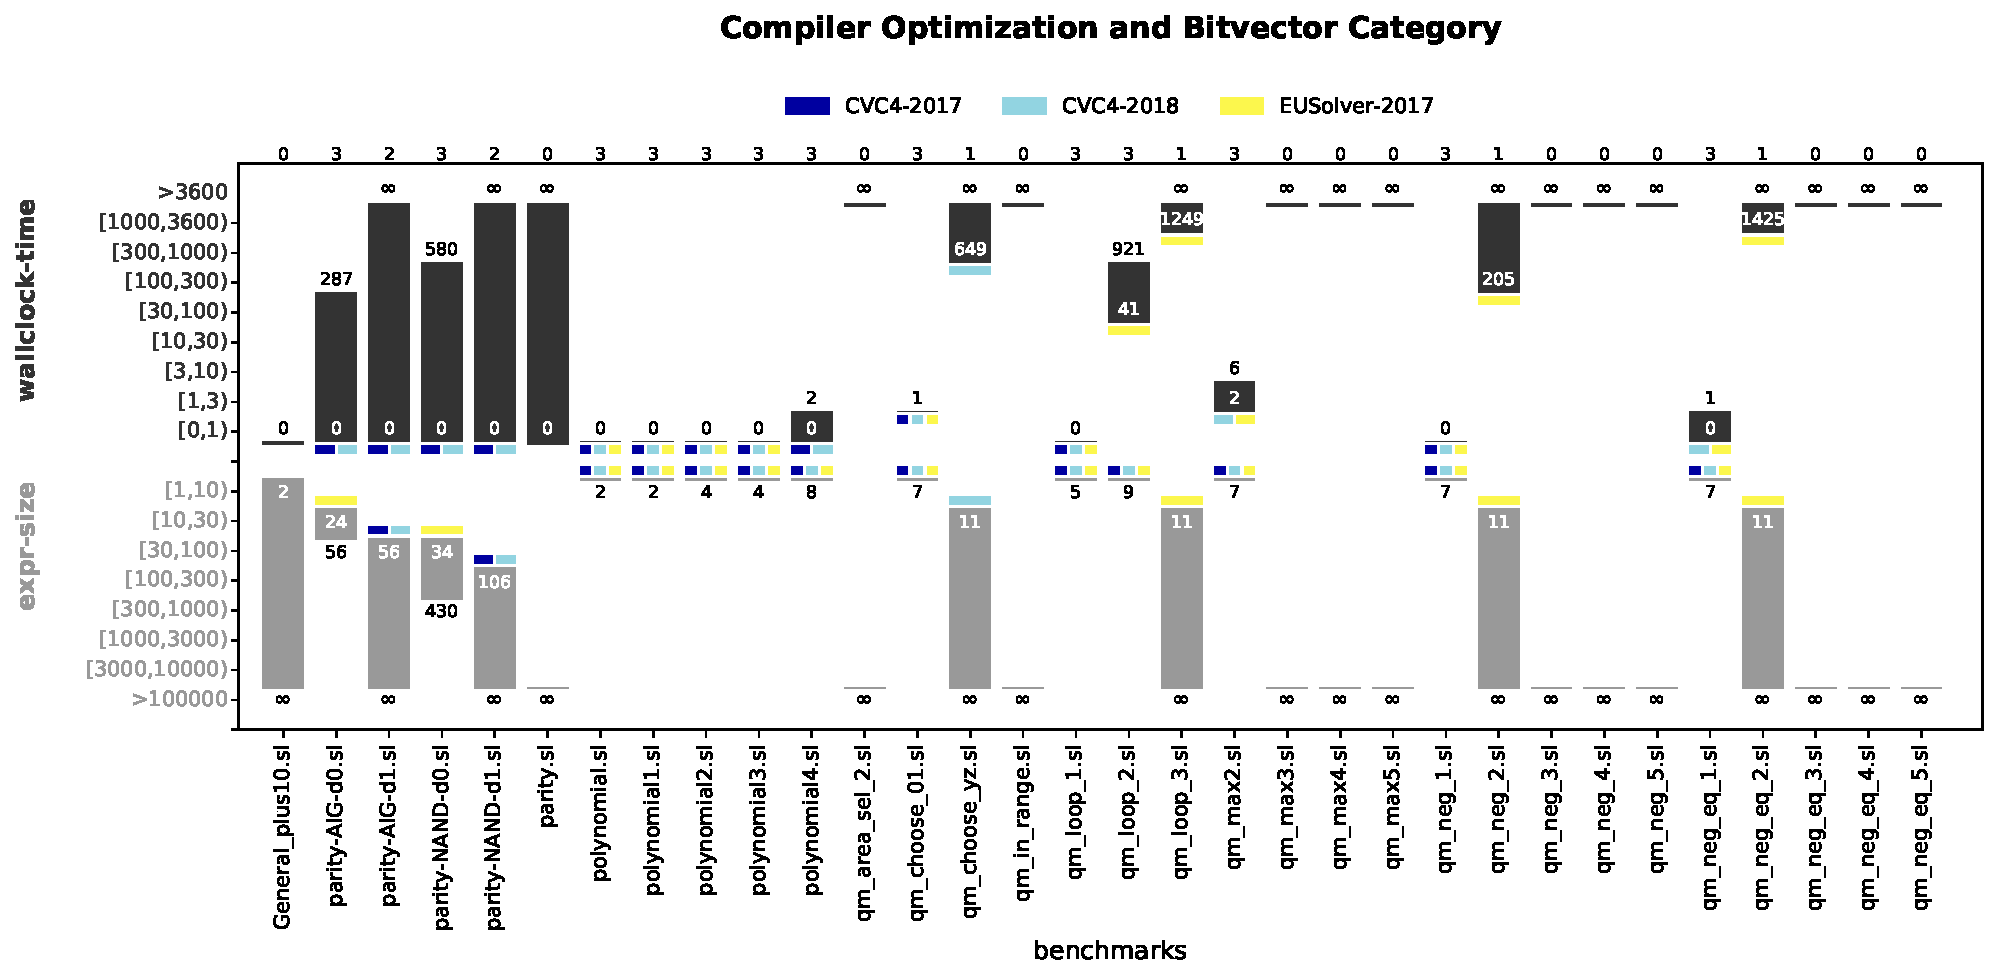
\includegraphics[width=10in]{figures/General1.pdf} \\[3cm]
				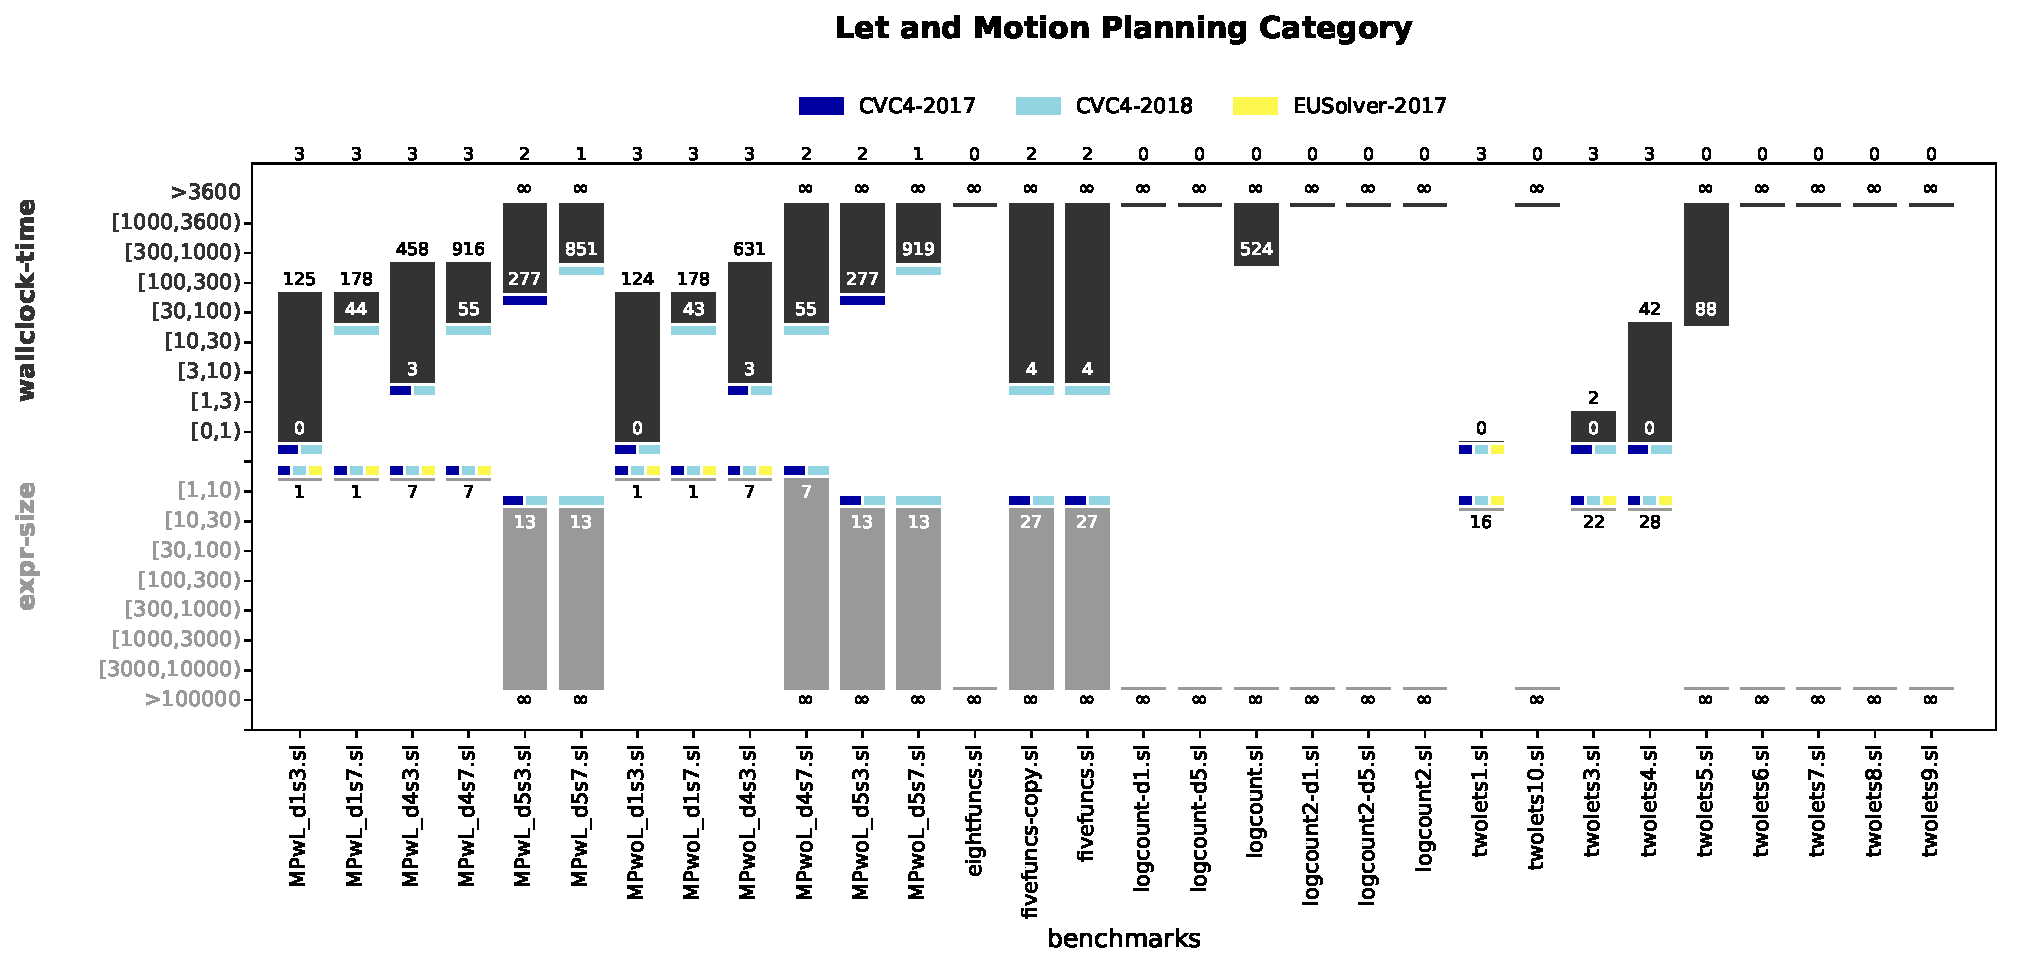
\includegraphics[width=10in]{figures/General2.pdf}
			\end{tabular}
	}}
	\caption{Evaluation of compiler optimizations, bitvectors, let and motion planning,
			 and program repair categories of the General track.}
	\label{fig:let-mot-plan}
\end{figure*}

\begin{figure*}
	\noindent\makebox[\textwidth]{
		\scalebox{0.625}{
			\begin{tabular}{c}
				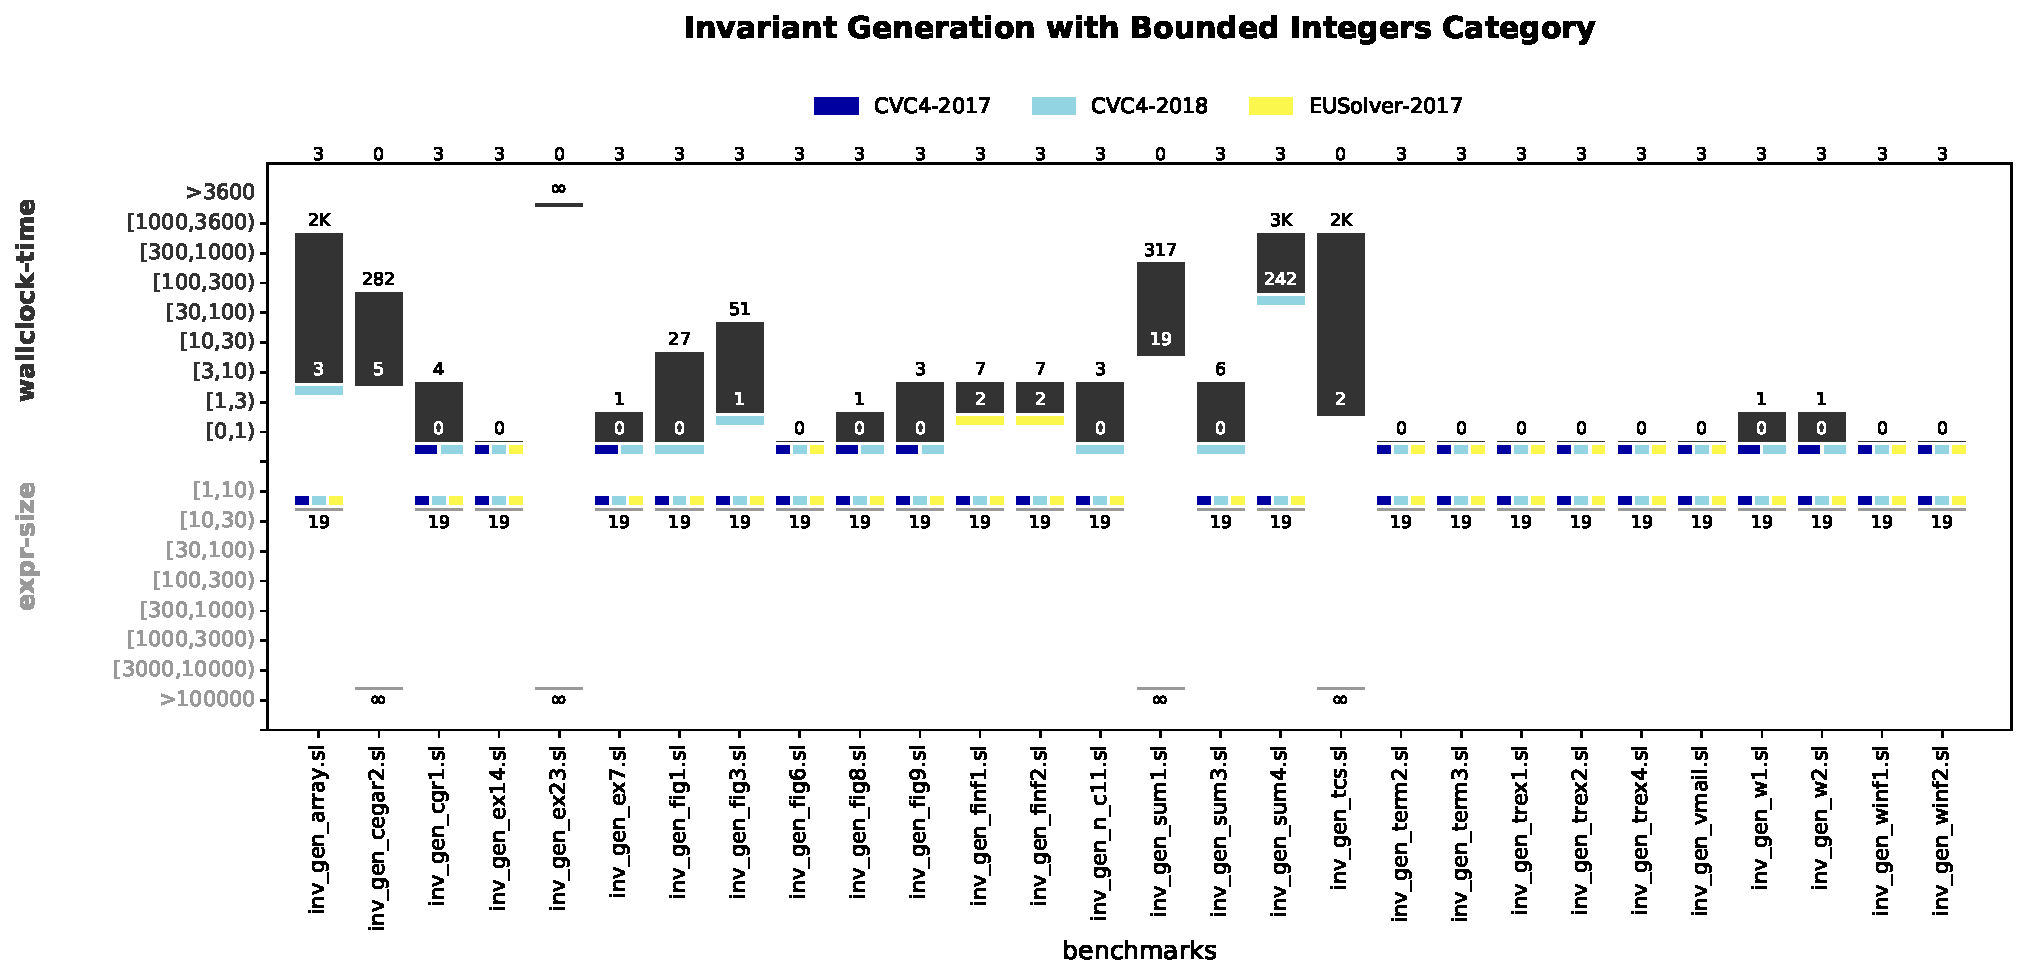
\includegraphics[width=10in]{figures/General3.pdf} \\[3cm]
				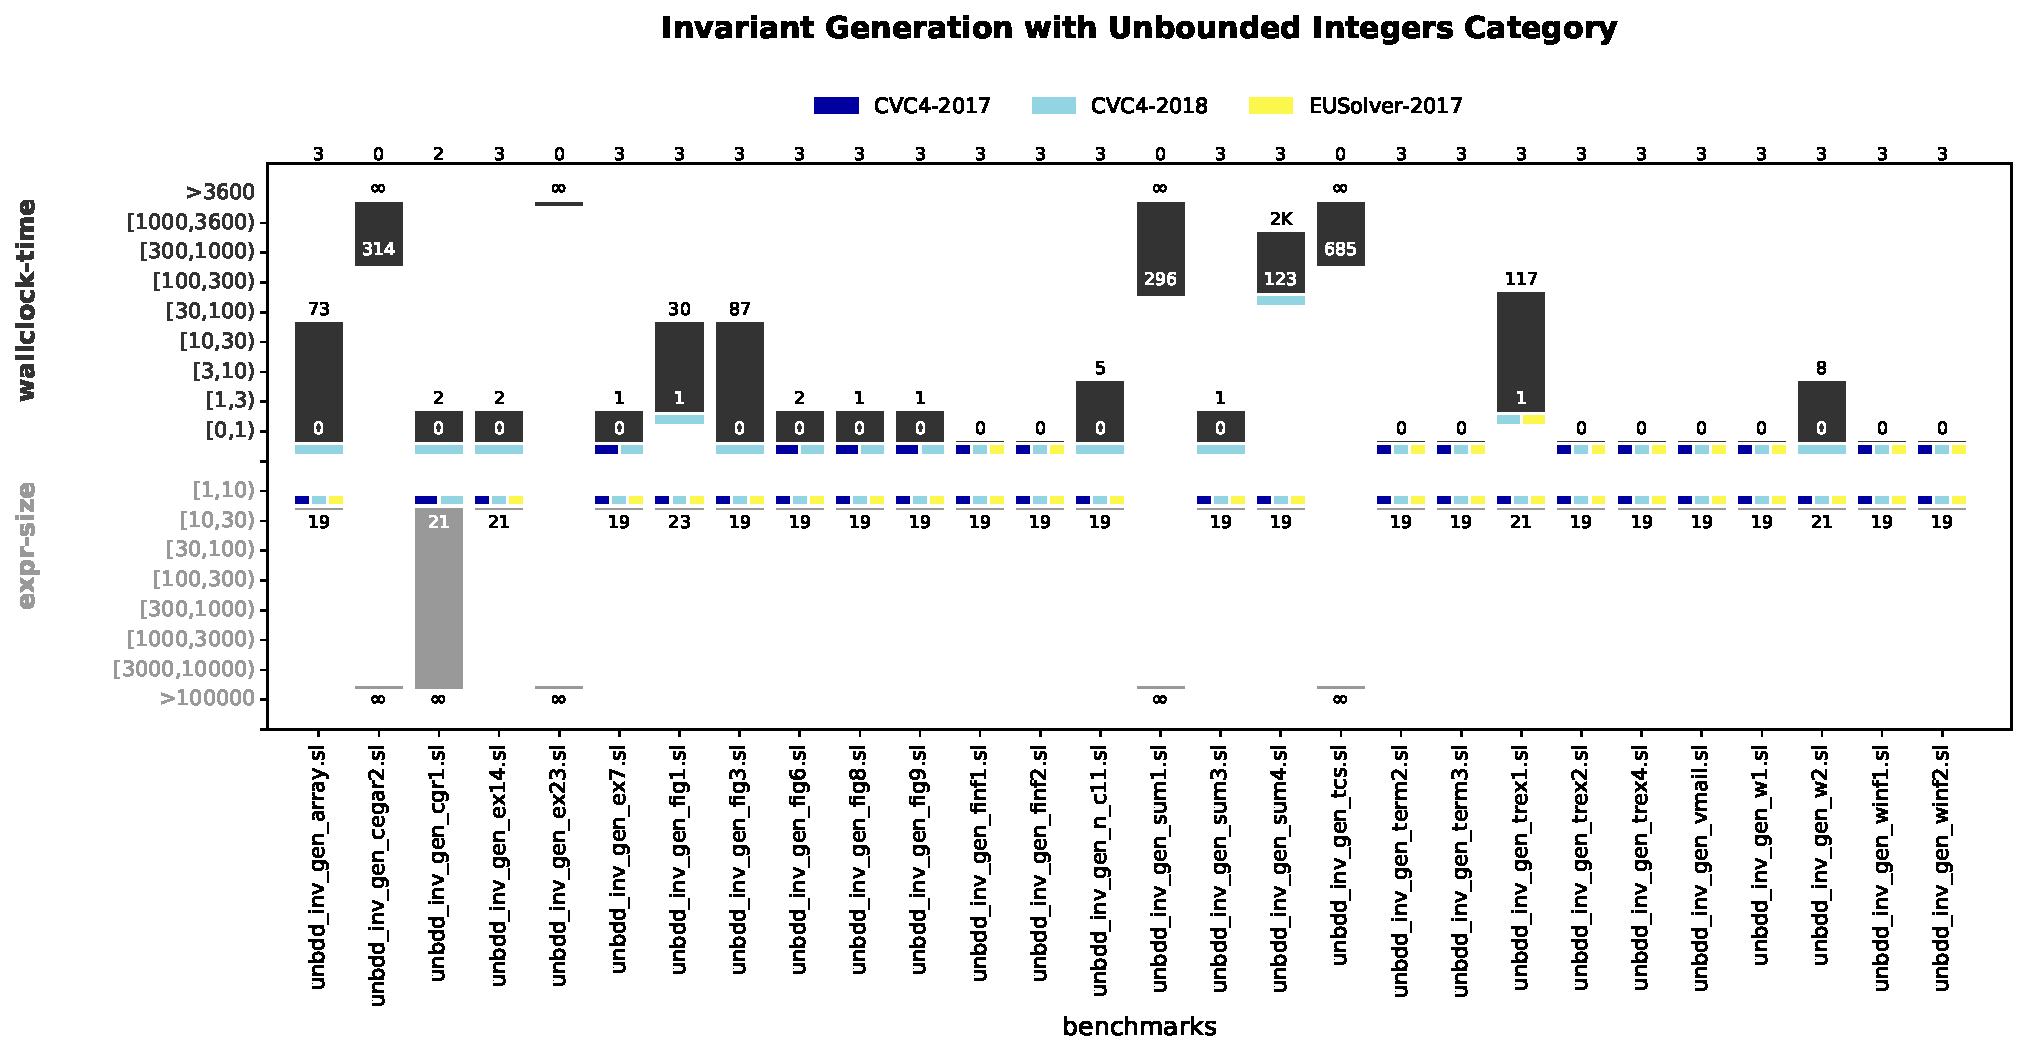
\includegraphics[width=10in]{figures/General4.pdf} 
			\end{tabular}
	}}
	\caption{Evaluation of invariant generation categories of the General track.}
	\label{fig:inv-results}
\end{figure*}

\begin{figure*}
	\noindent\makebox[\textwidth]{
		\scalebox{0.625}{
			\begin{tabular}{c}
				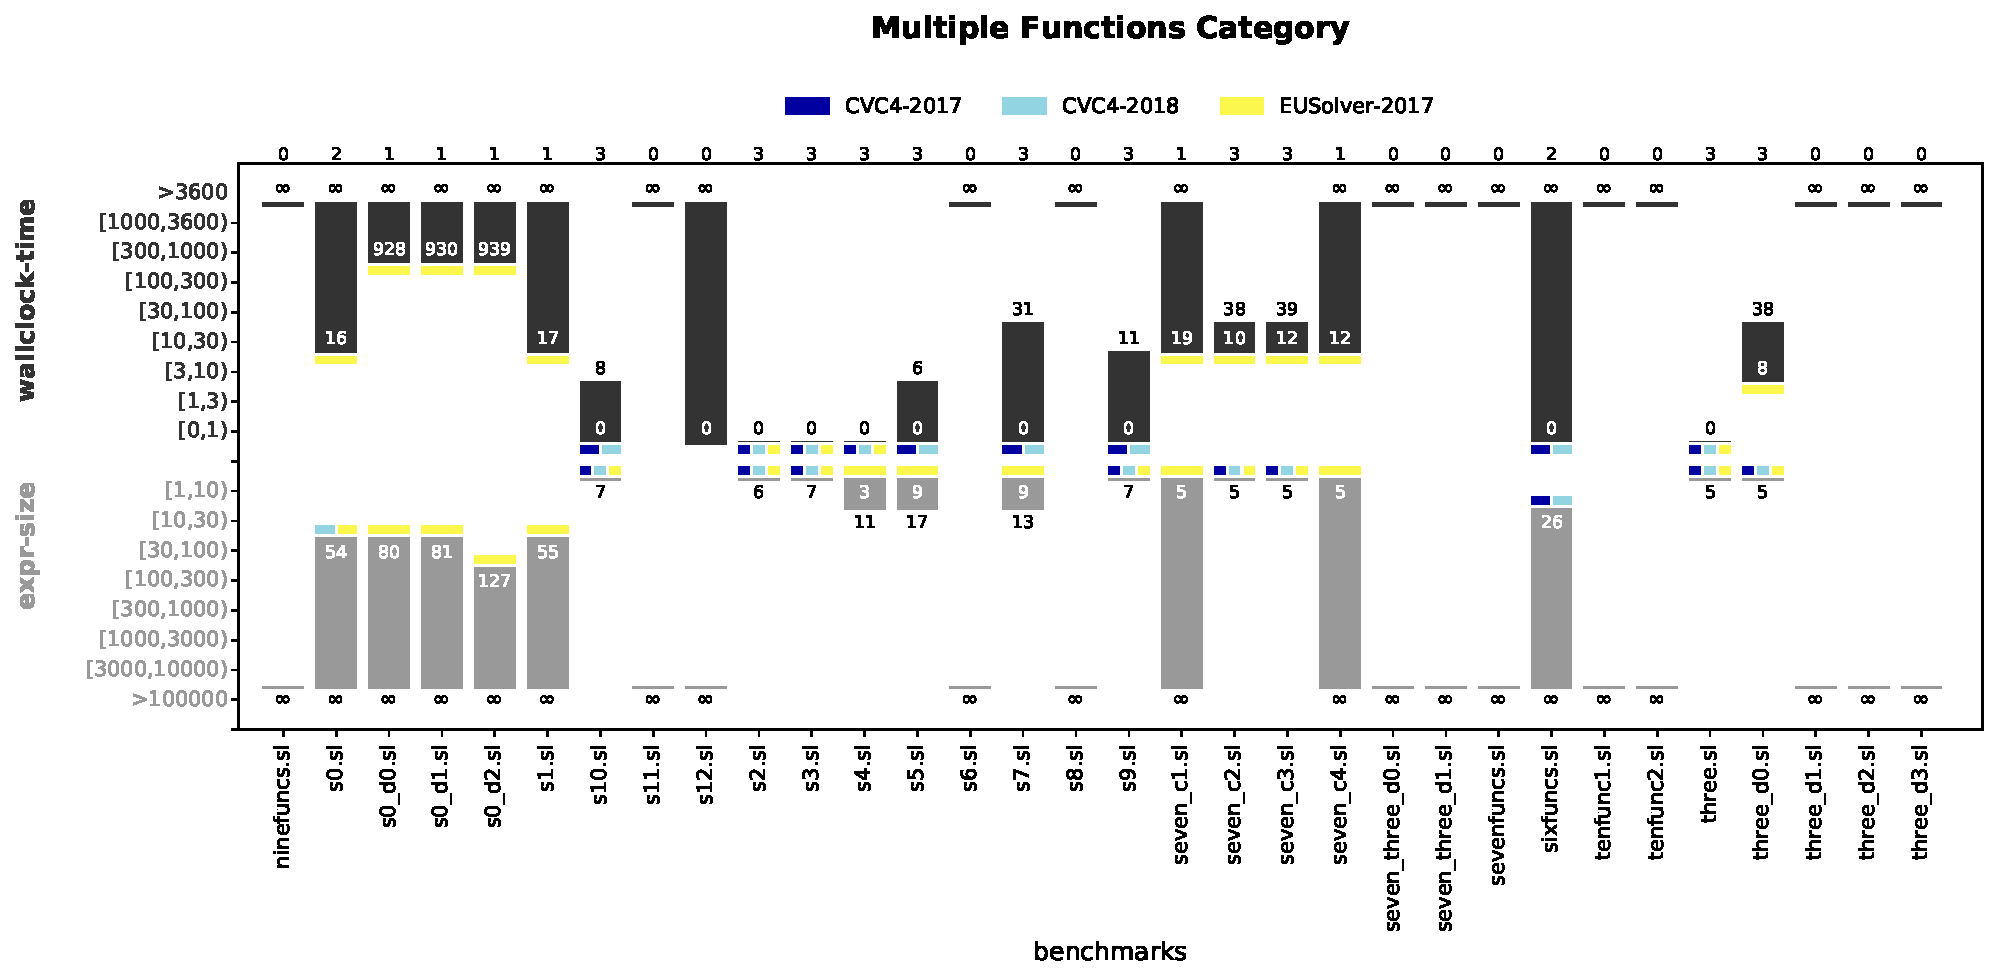
\includegraphics[width=10in]{figures/General5.pdf} \\[3cm]
				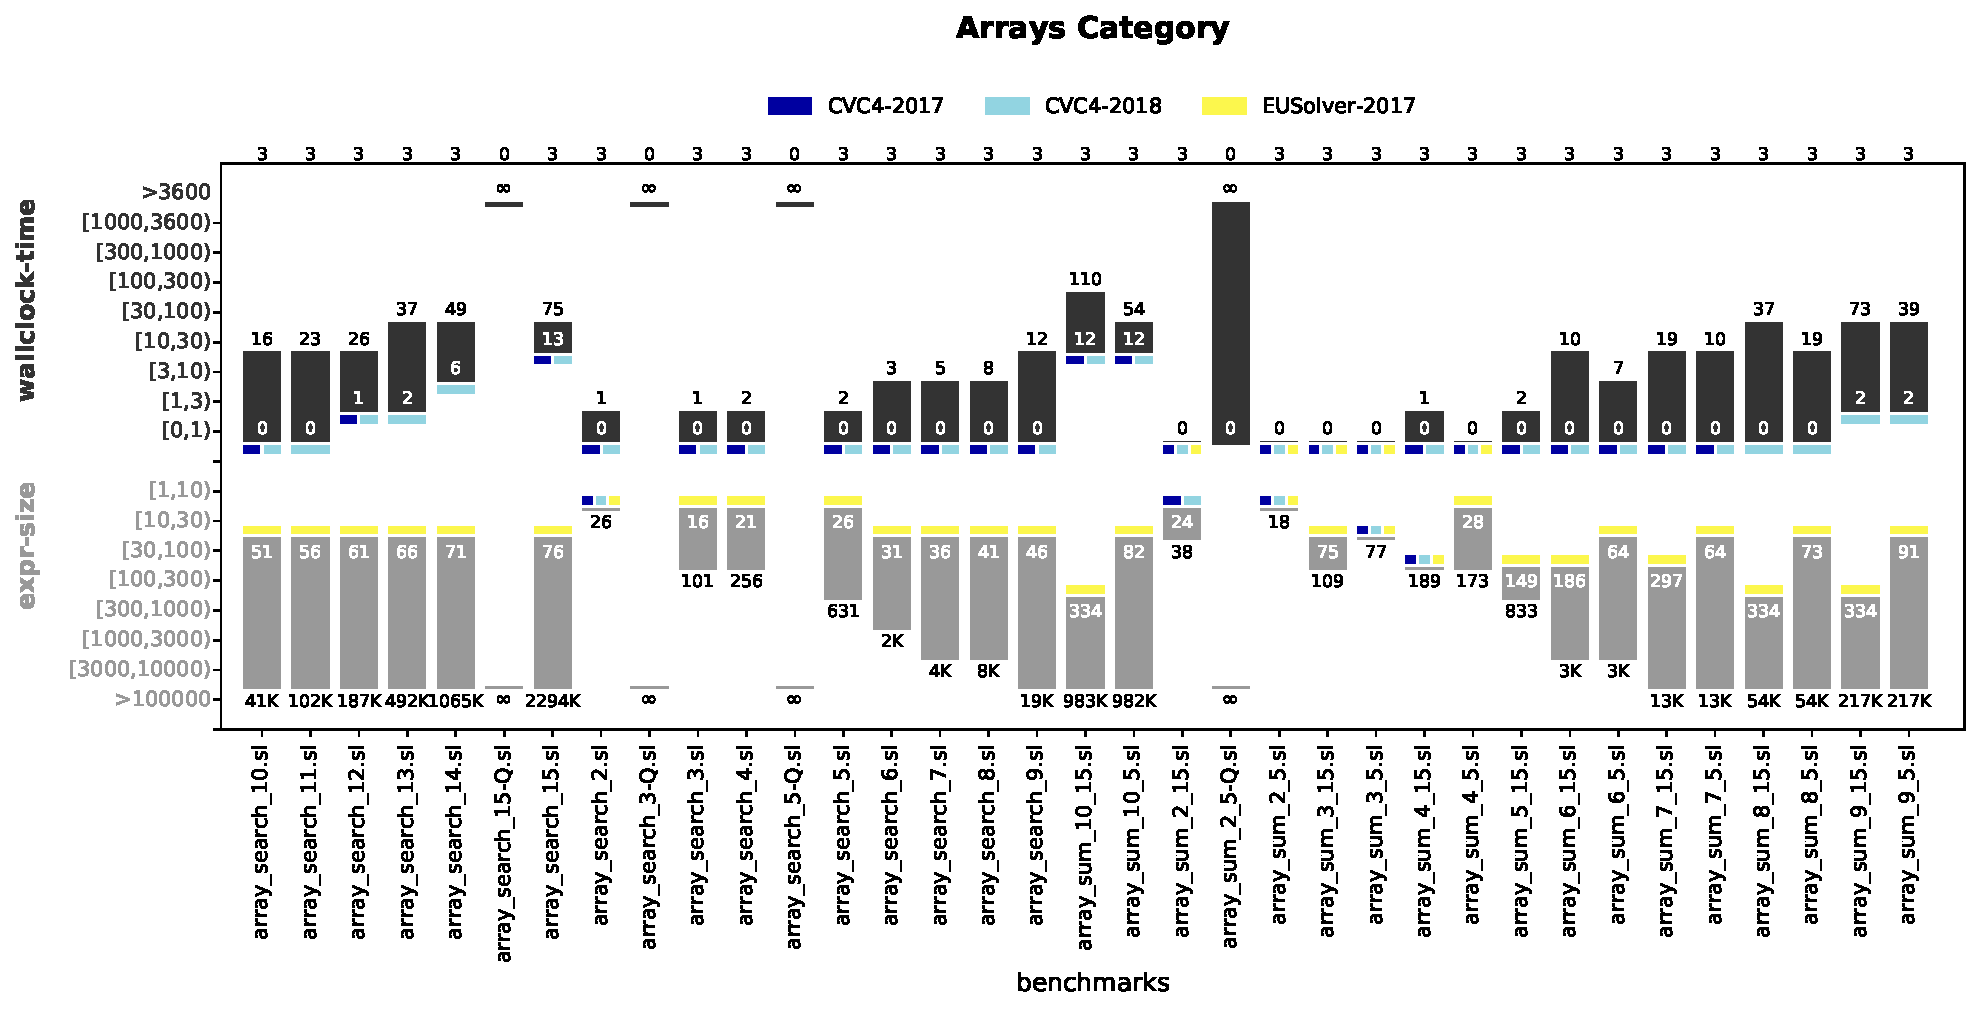
\includegraphics[width=10in]{figures/General6.pdf} 
			\end{tabular}
	}}
	\caption{Evaluation of multiple functions and arrays categories of the General track.}
	\label{fig:mult-func-arr}
\end{figure*}

\begin{figure*}
	\noindent\makebox[\textwidth]{
		\scalebox{0.6}{
			\begin{tabular}{c}
				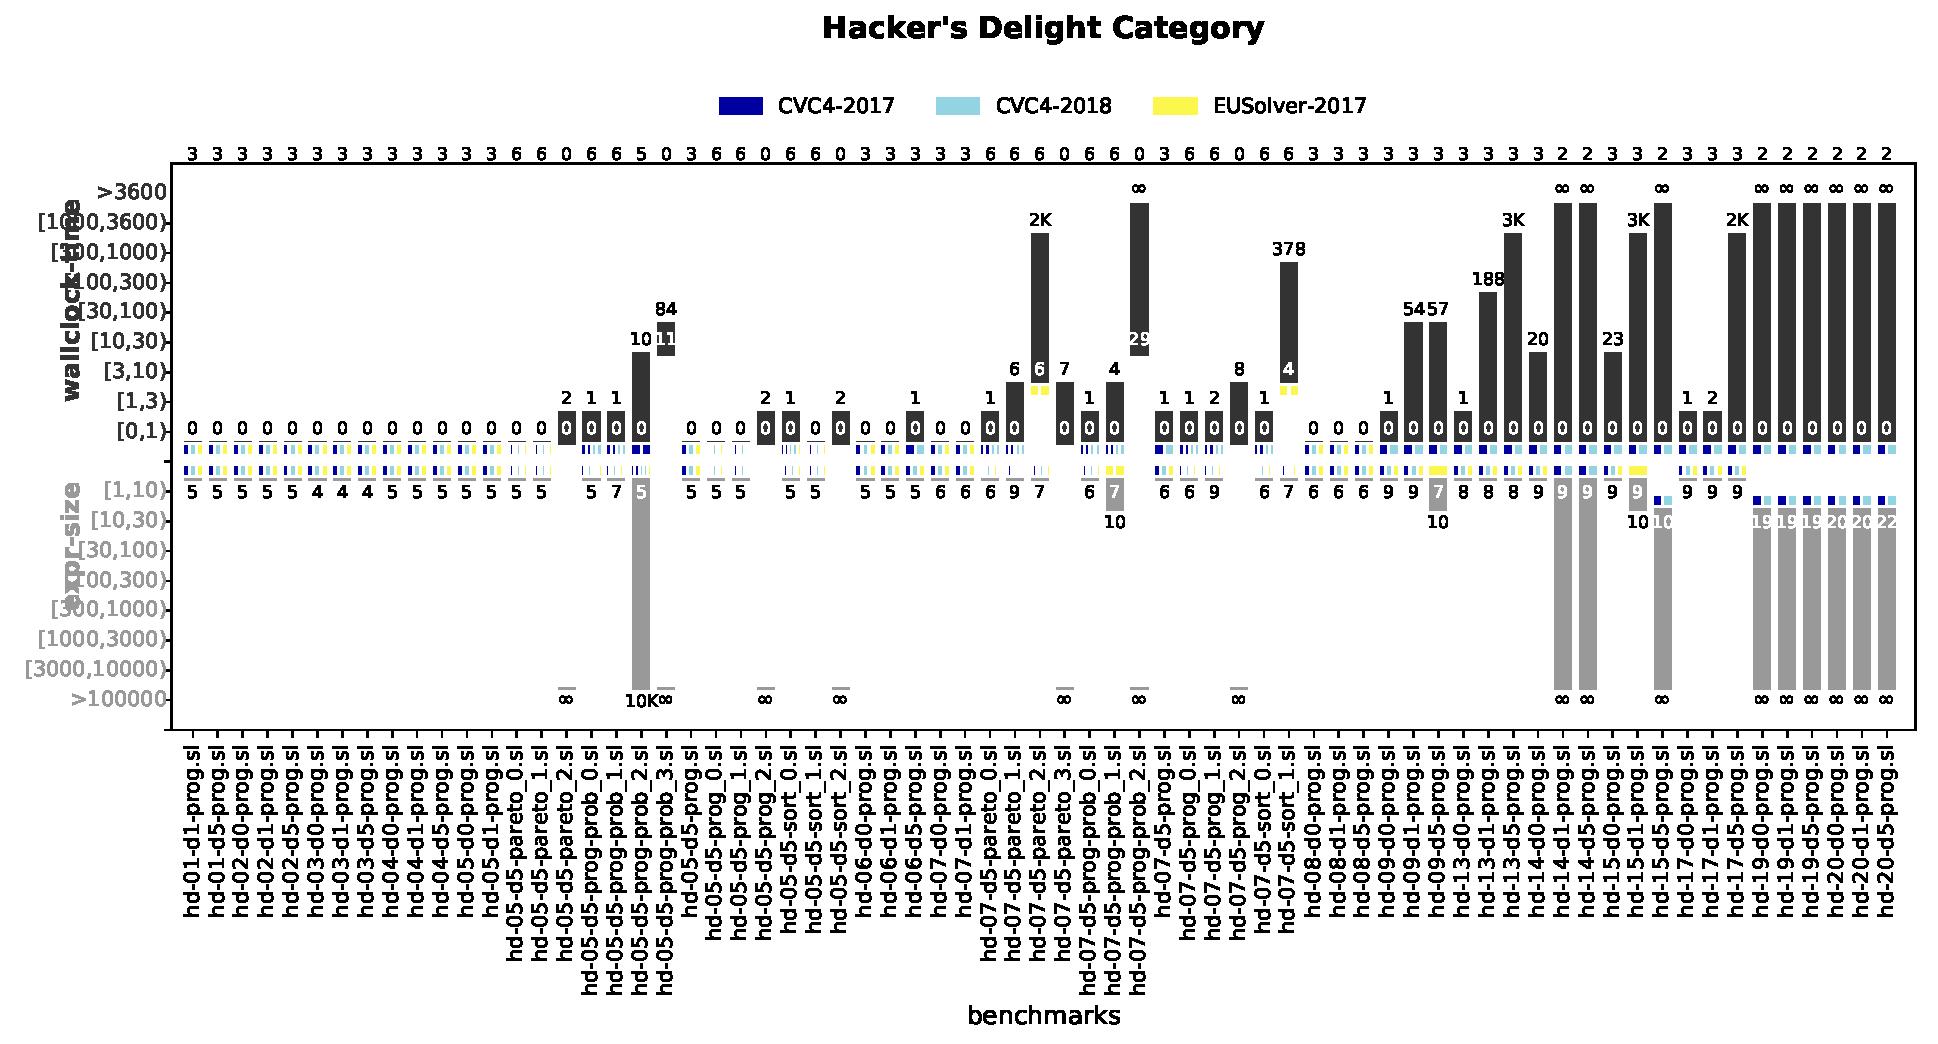
\includegraphics[width=10in]{figures/General7.pdf} \\[3cm]
				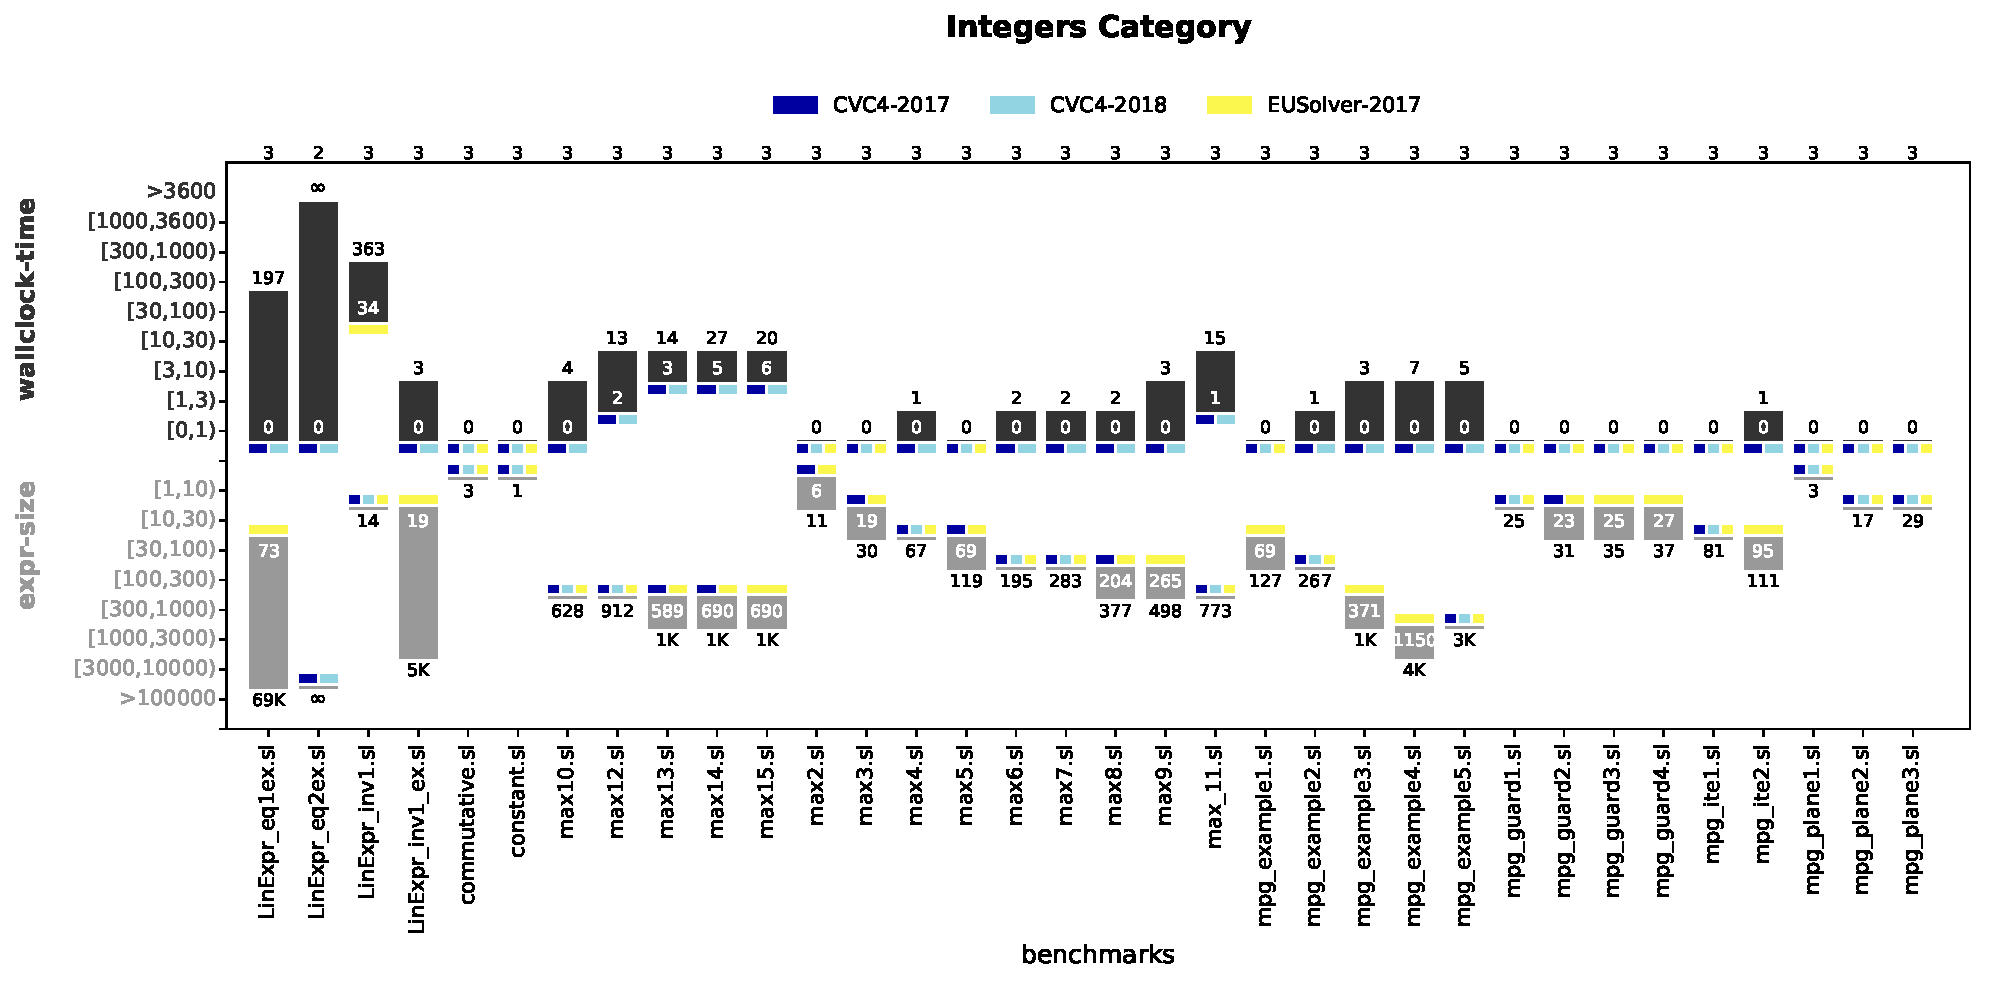
\includegraphics[width=10in]{figures/General8.pdf} 
			\end{tabular}
	}}
	\caption{Evaluation of hacker's delight and integers categories of the General track.}
	\label{fig:hd-int}
\end{figure*}

\begin{figure*}
	\noindent\makebox[\textwidth]{
		\scalebox{0.625}{
			\begin{tabular}{c}
				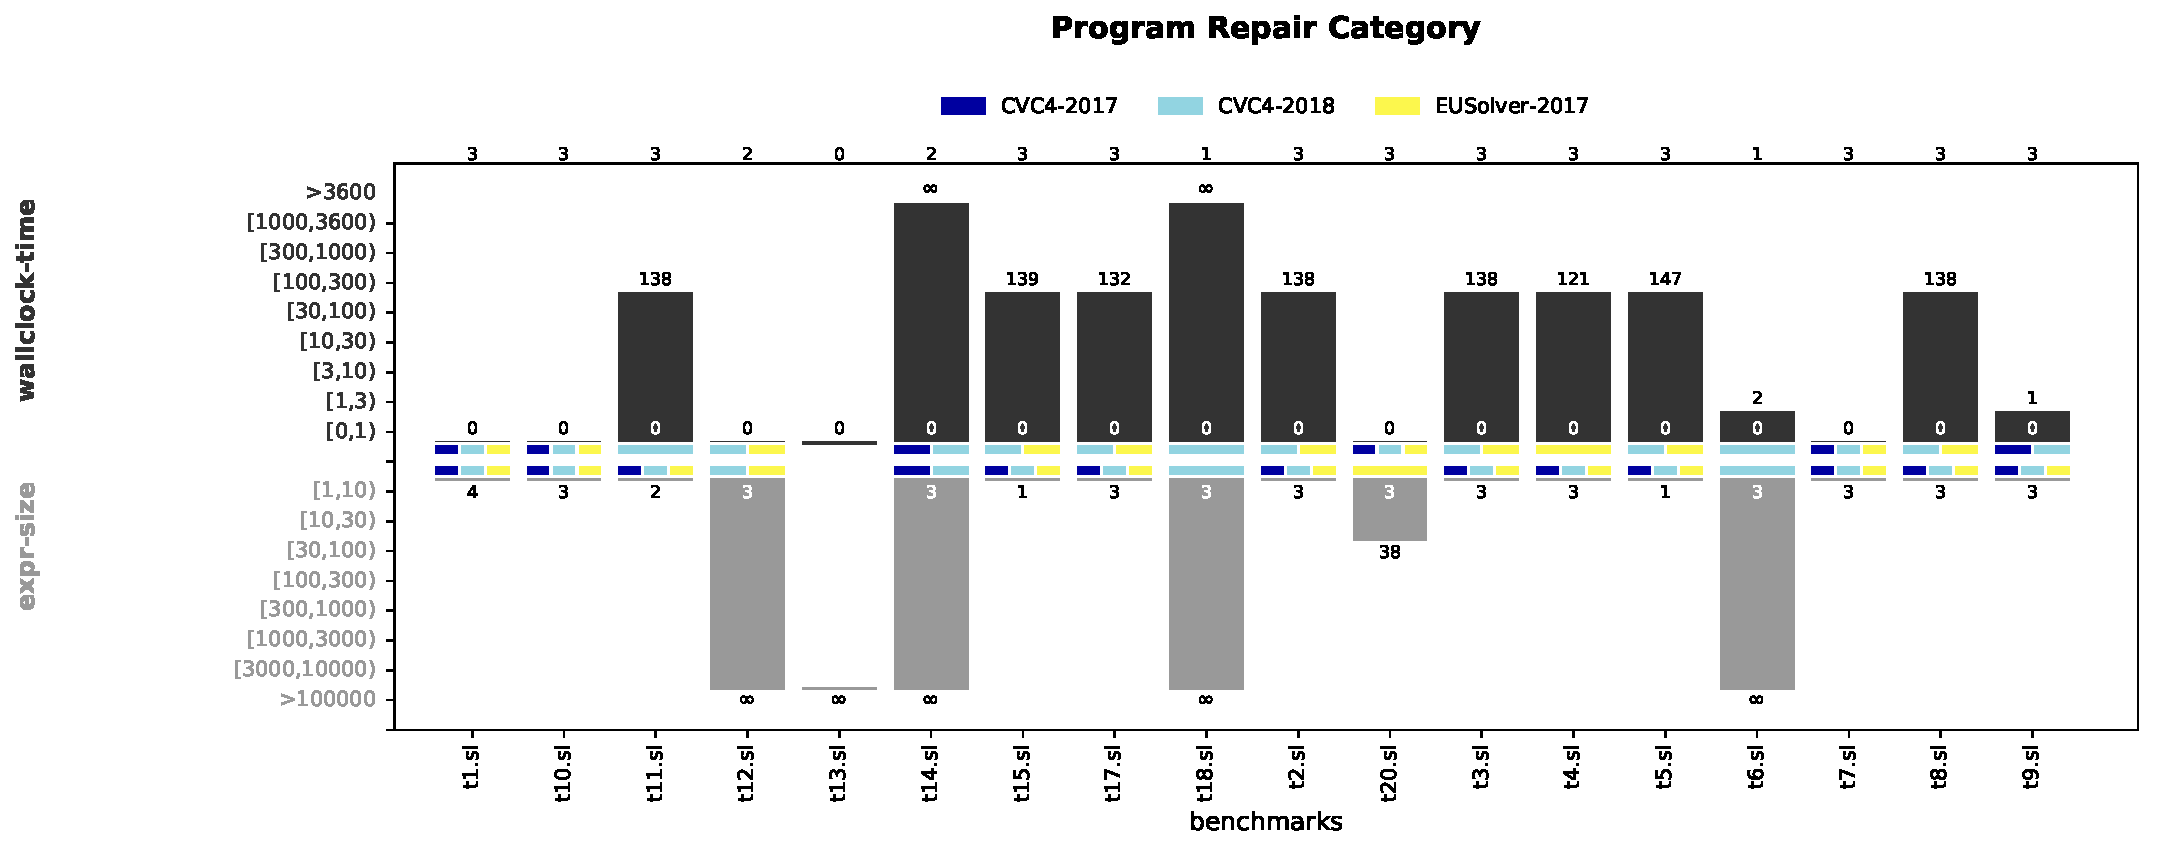
\includegraphics[width=10in]{figures/General9.pdf} \\[3cm]
				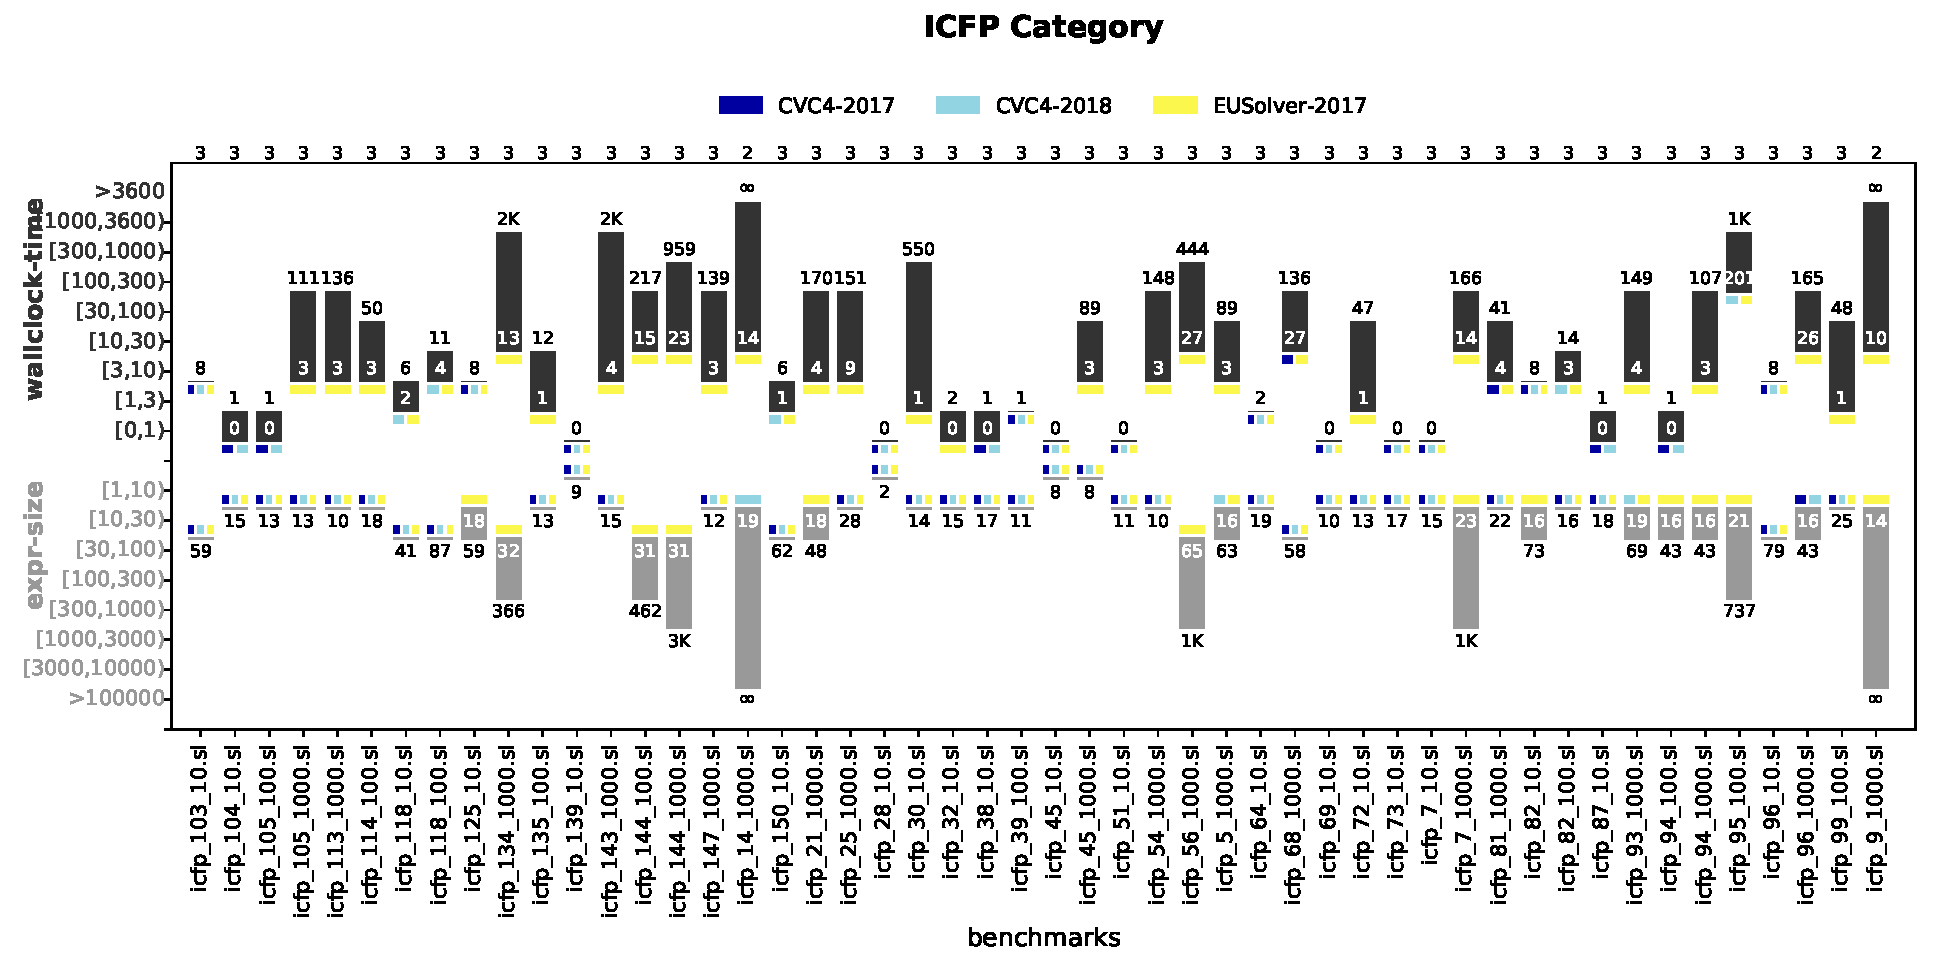
\includegraphics[width=10in]{figures/General10.pdf}
			\end{tabular}
	}}
	\caption{Evaluation of program repair and ICFP categories of the General track.}
	\label{fig:prog-rep-icfp}
\end{figure*}

\begin{figure*}
	\noindent\makebox[\textwidth]{
		\scalebox{0.625}{
			\begin{tabular}{c}
				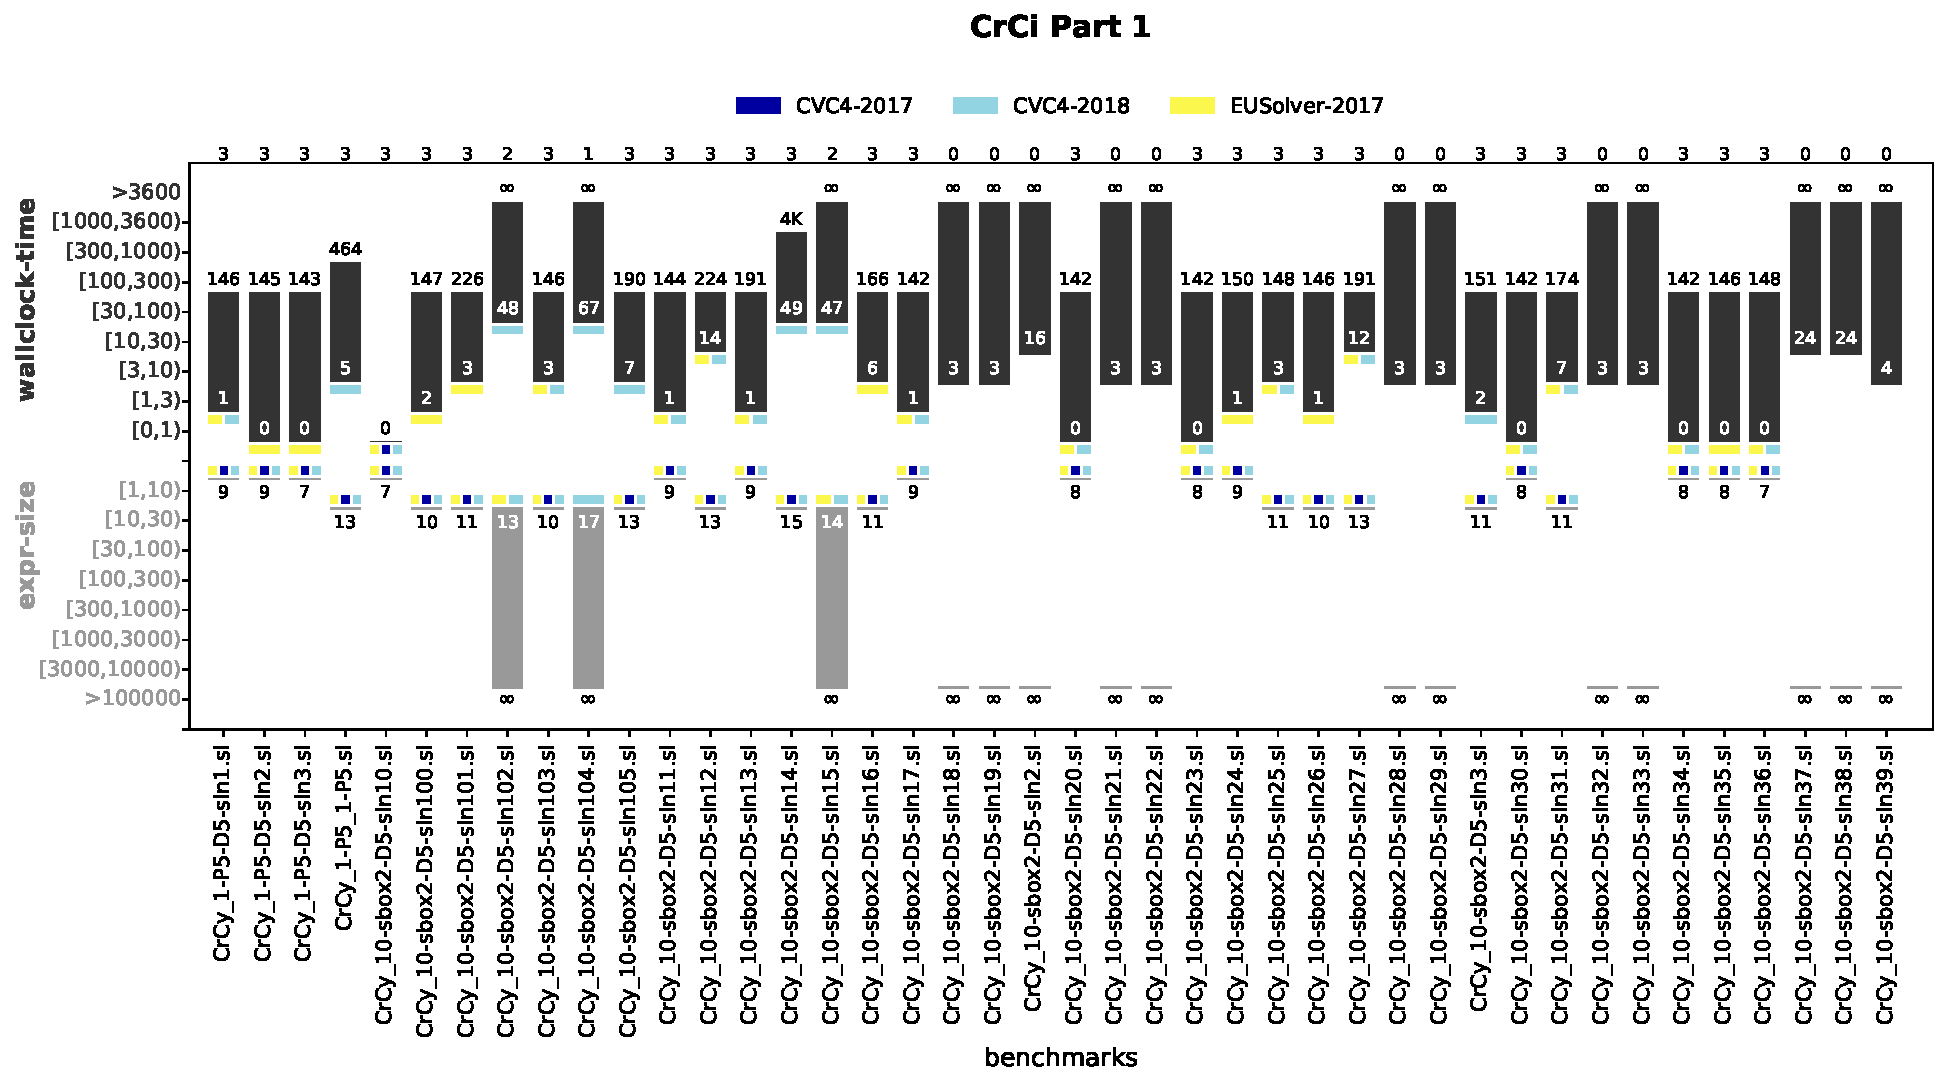
\includegraphics[width=10in]{figures/CrCi1.pdf} \\[3cm]
				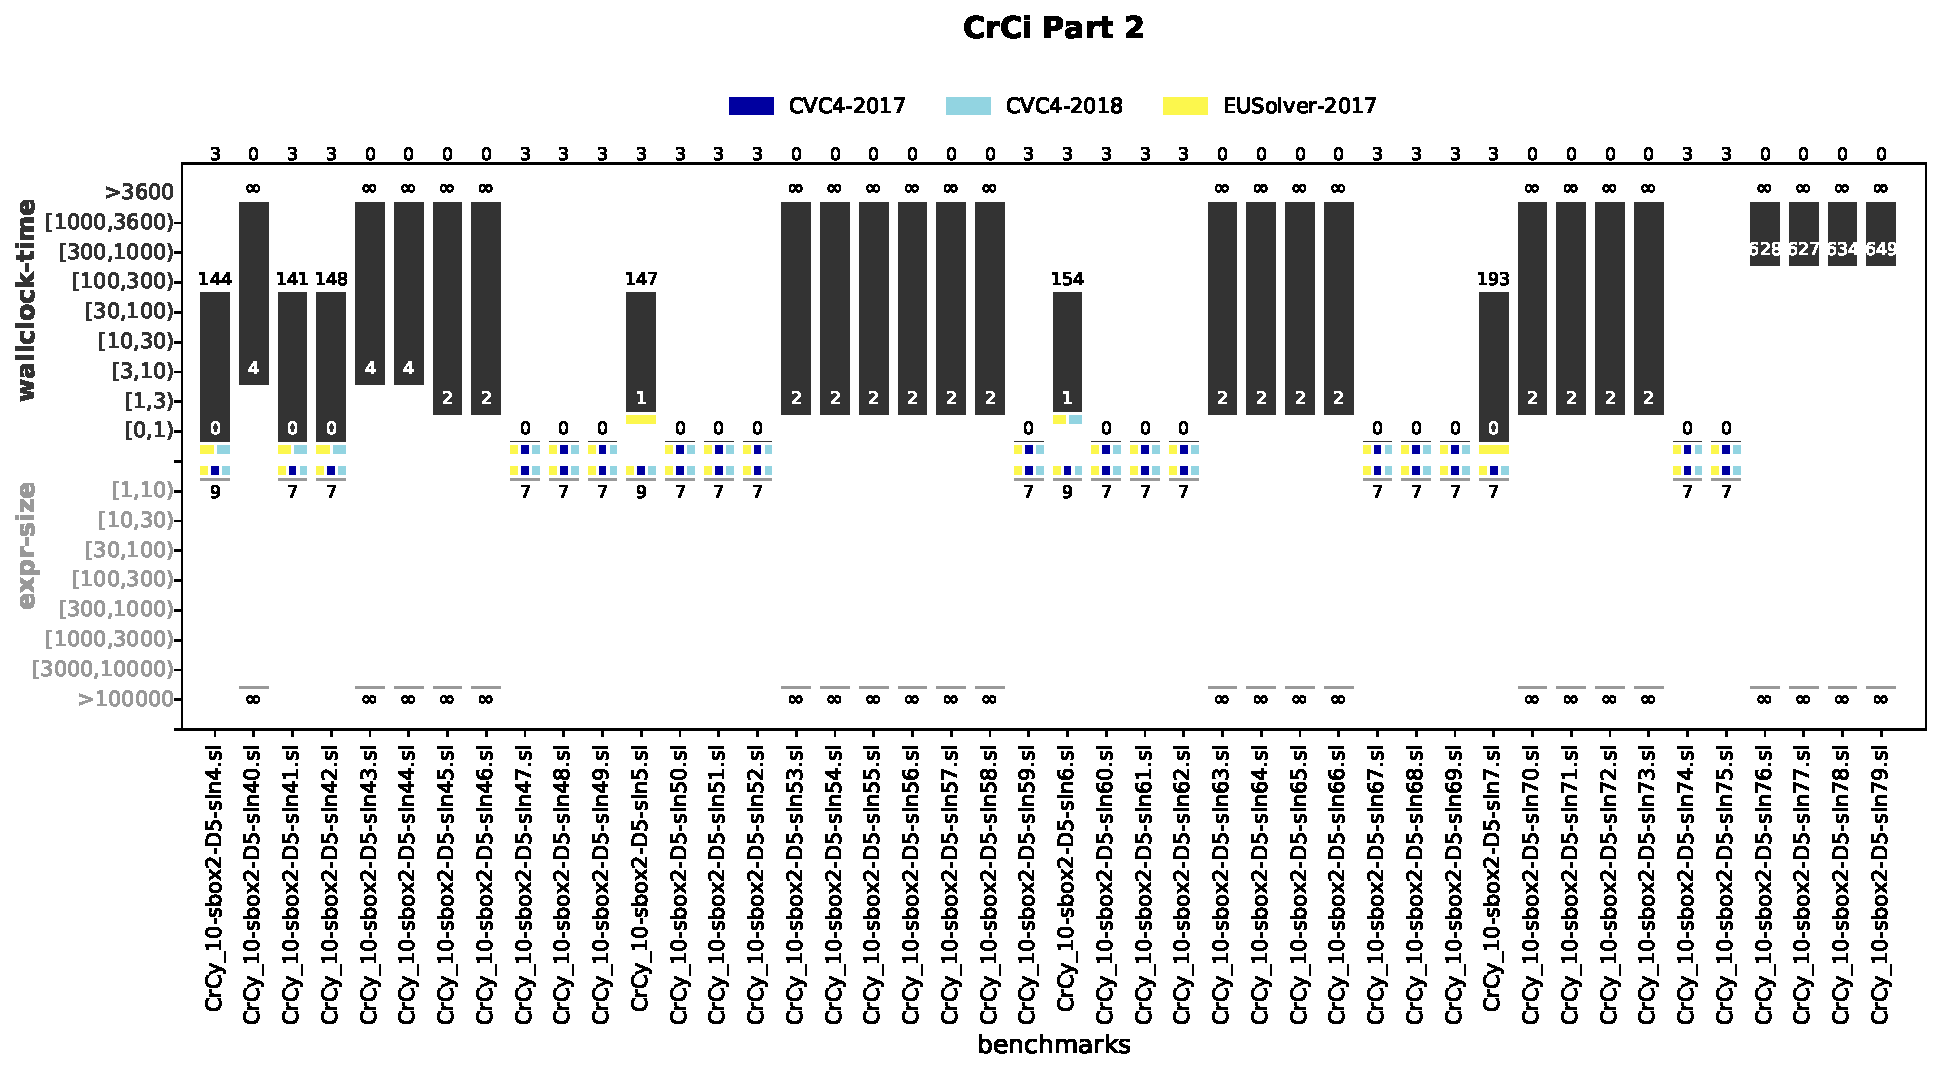
\includegraphics[width=10in]{figures/CrCi2.pdf}
			\end{tabular}
	}}
	\caption{Evaluation of crypto circuits category of the General track (Parts 1 \& 2).}
	\label{fig:crci-1}
\end{figure*}

\begin{figure*}
	\noindent\makebox[\textwidth]{
		\scalebox{0.625}{
			\begin{tabular}{c}
				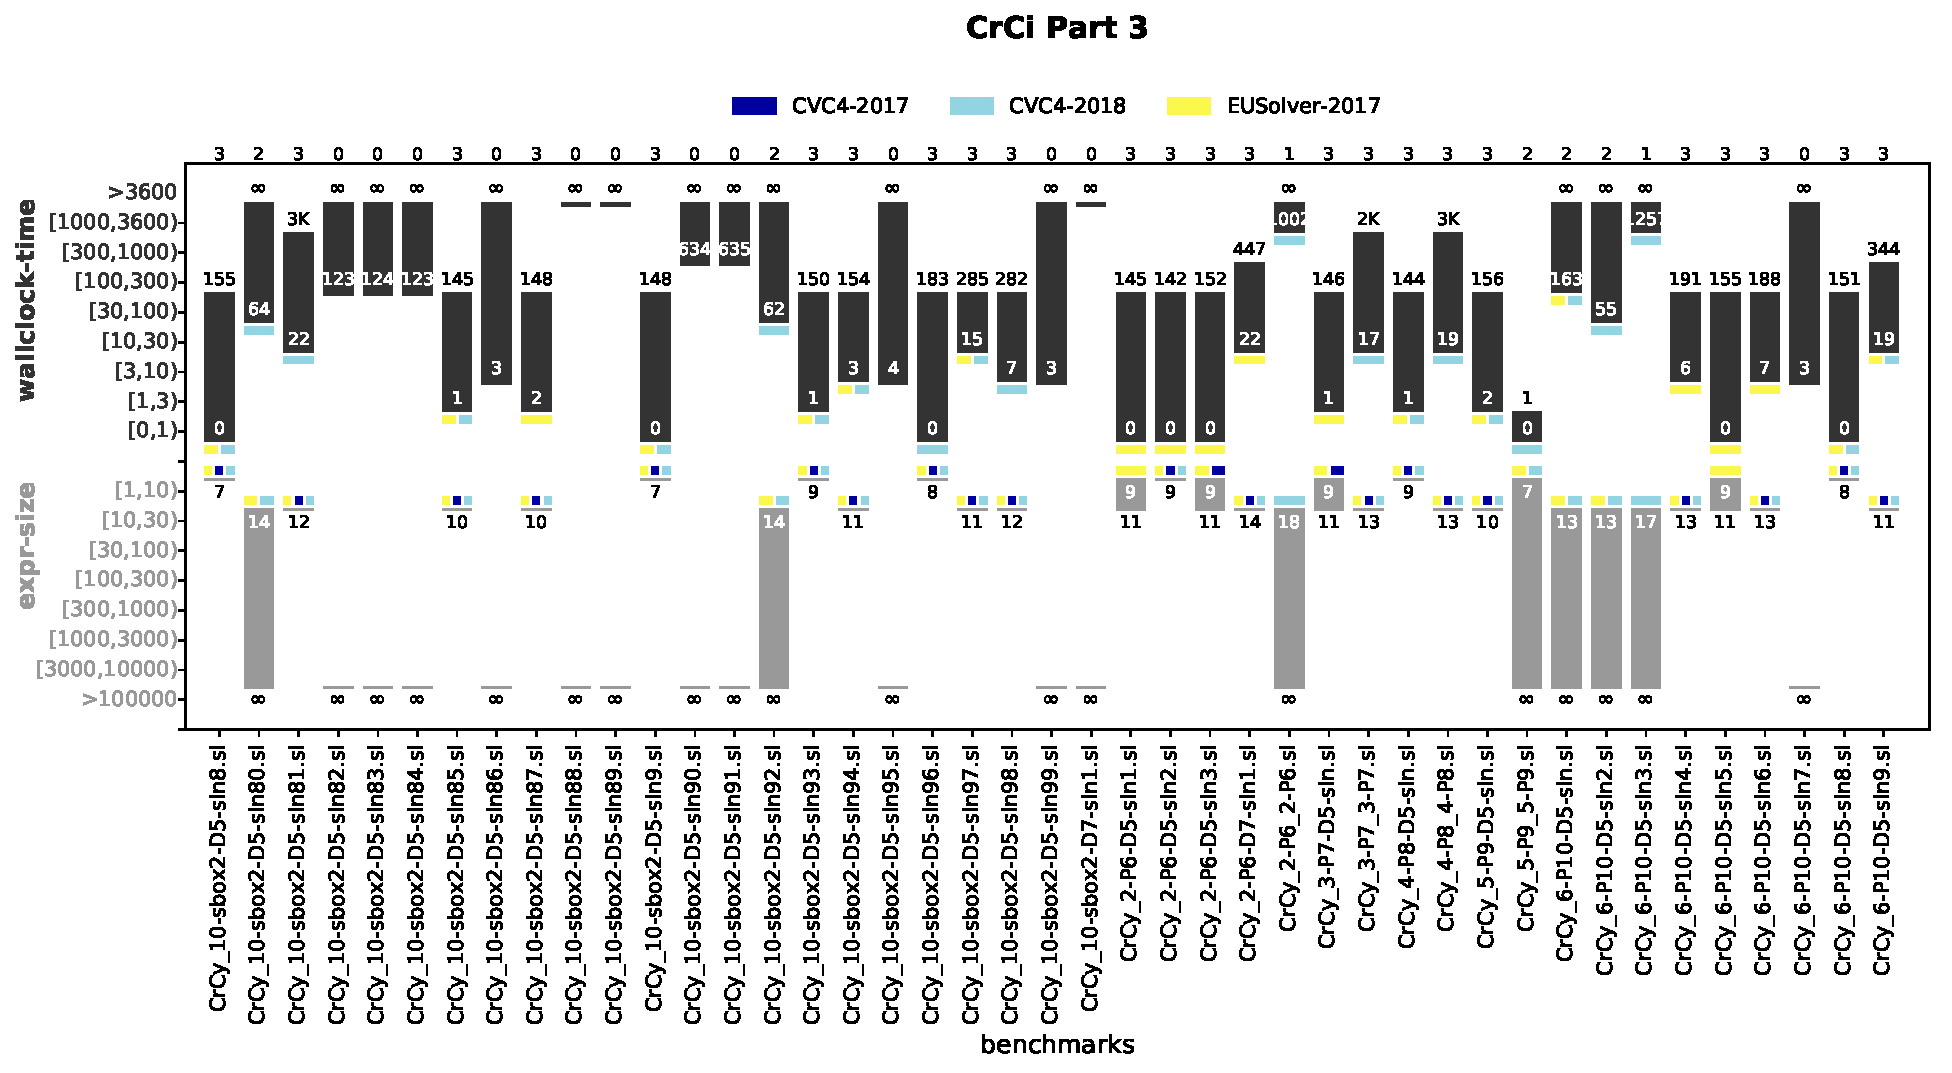
\includegraphics[width=10in]{figures/CrCi3.pdf} \\[3cm]
				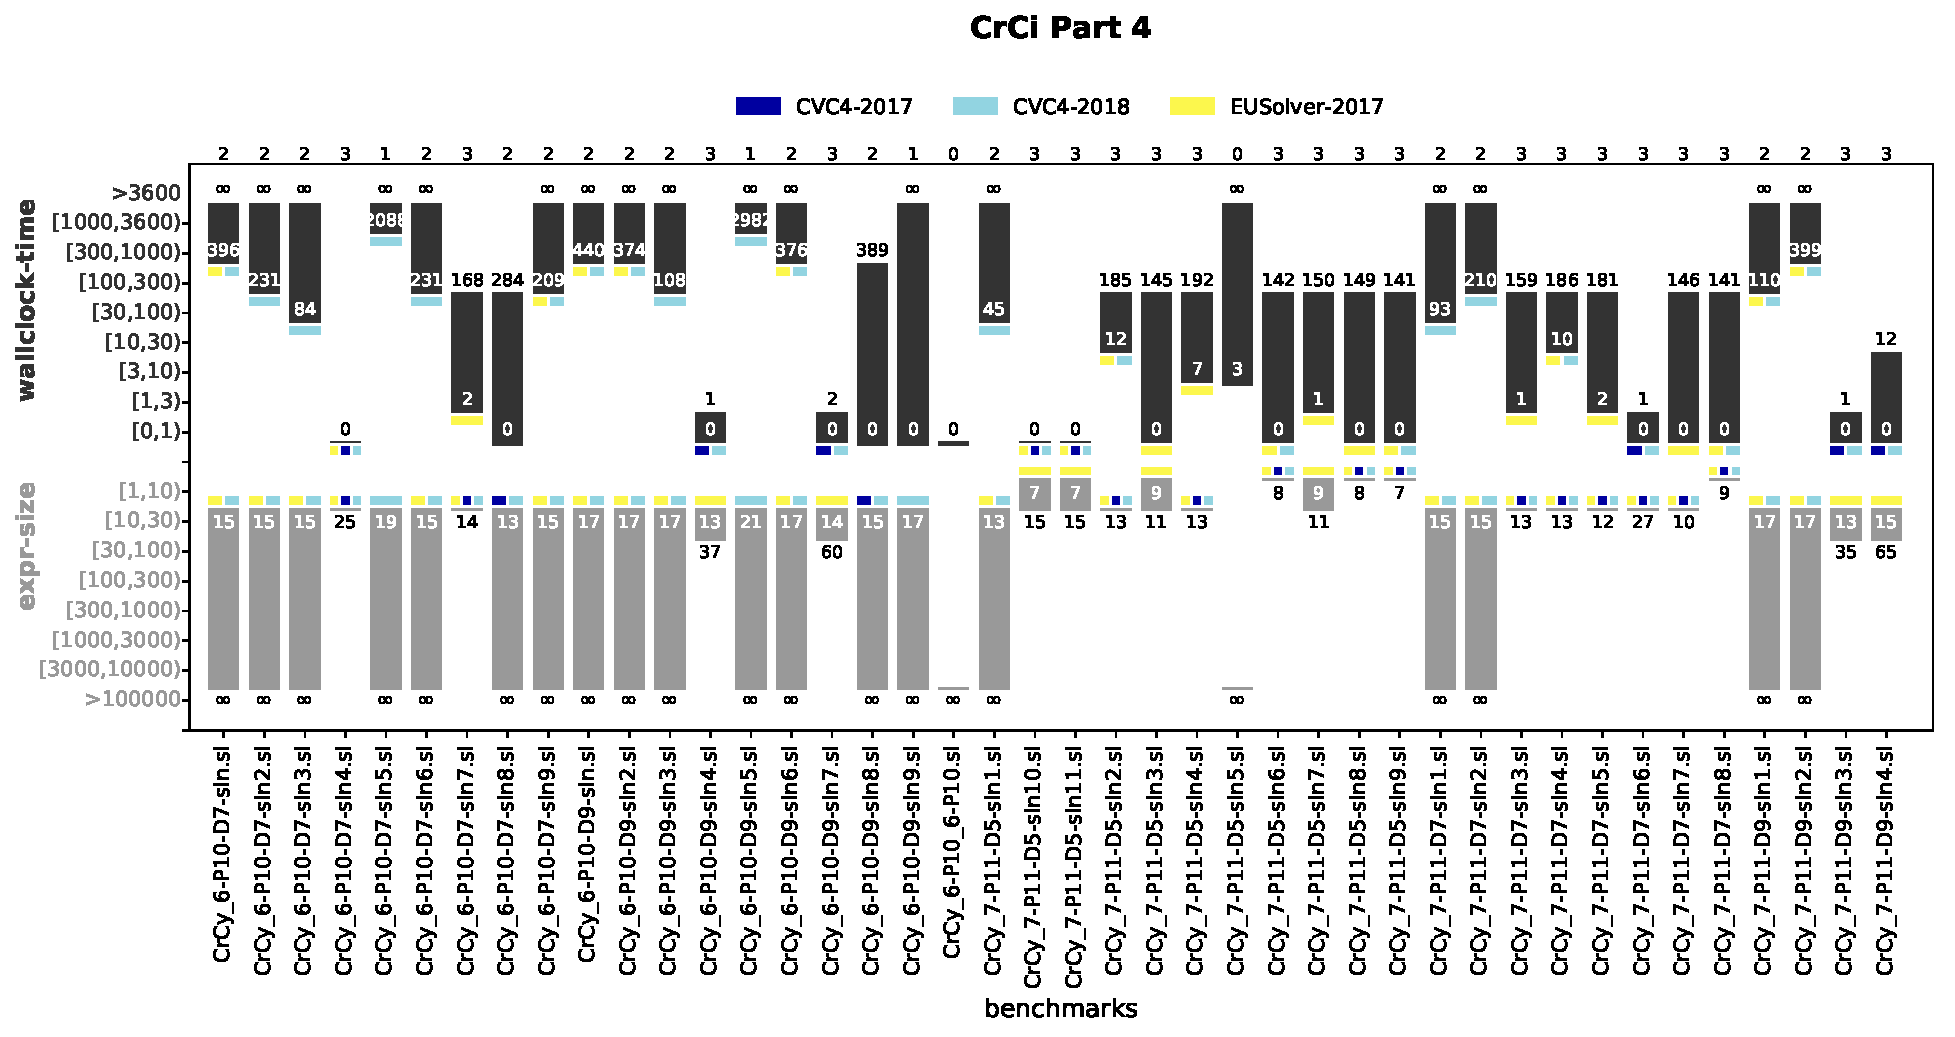
\includegraphics[width=10in]{figures/CrCi4.pdf}
			\end{tabular}
	}}
	\caption{Evaluation of crypto circuits category of the General track (Parts 3 \& 4).}
	\label{fig:crci-2}
\end{figure*}
	
\begin{figure*}
	\noindent\makebox[\textwidth]{
		\scalebox{0.625}{
			\begin{tabular}{c}
				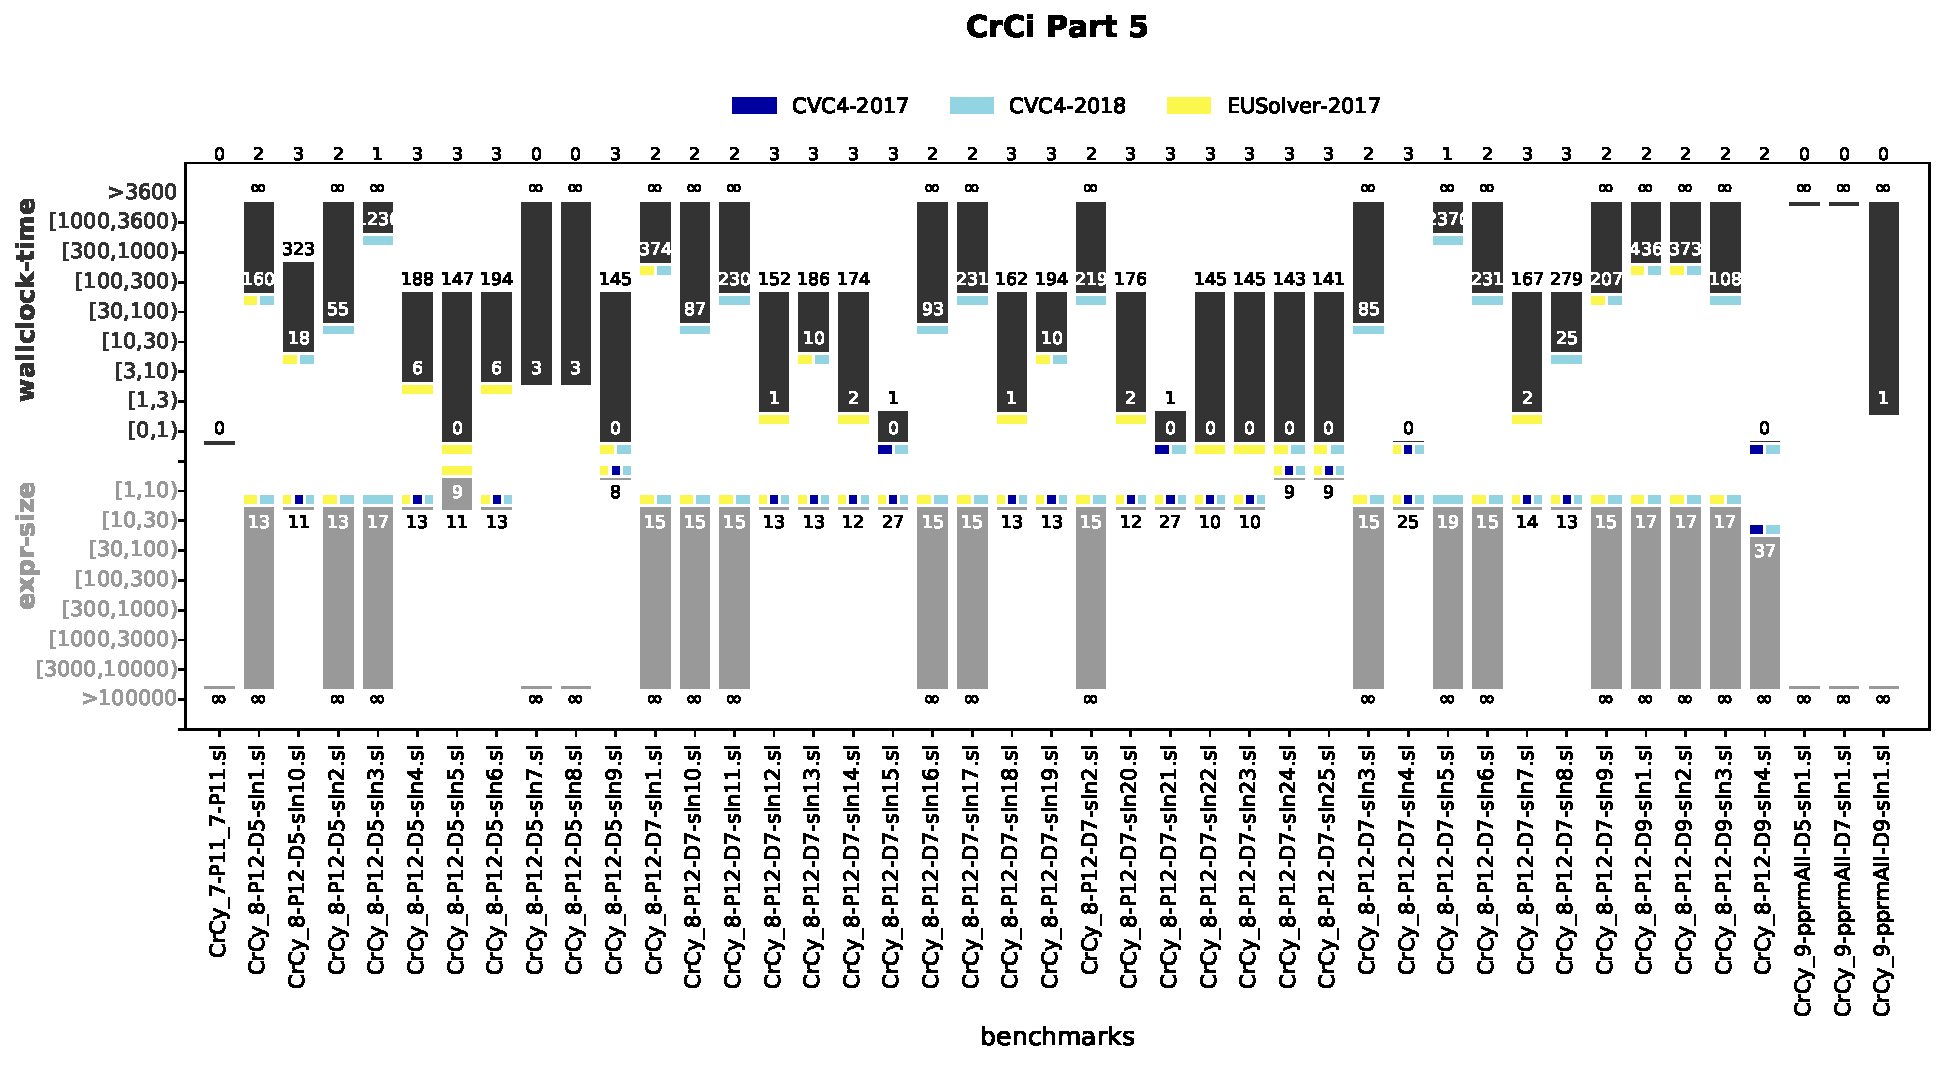
\includegraphics[width=10in]{figures/CrCi5.pdf}
			\end{tabular}
	}}
	\caption{Evaluation of crypto circuits category of the General track (Part 5).}
	\label{fig:crci-5}
\end{figure*}
	

\begin{figure*}
	\noindent\makebox[\textwidth]{
		\scalebox{0.6}{
			\begin{tabular}{c}
				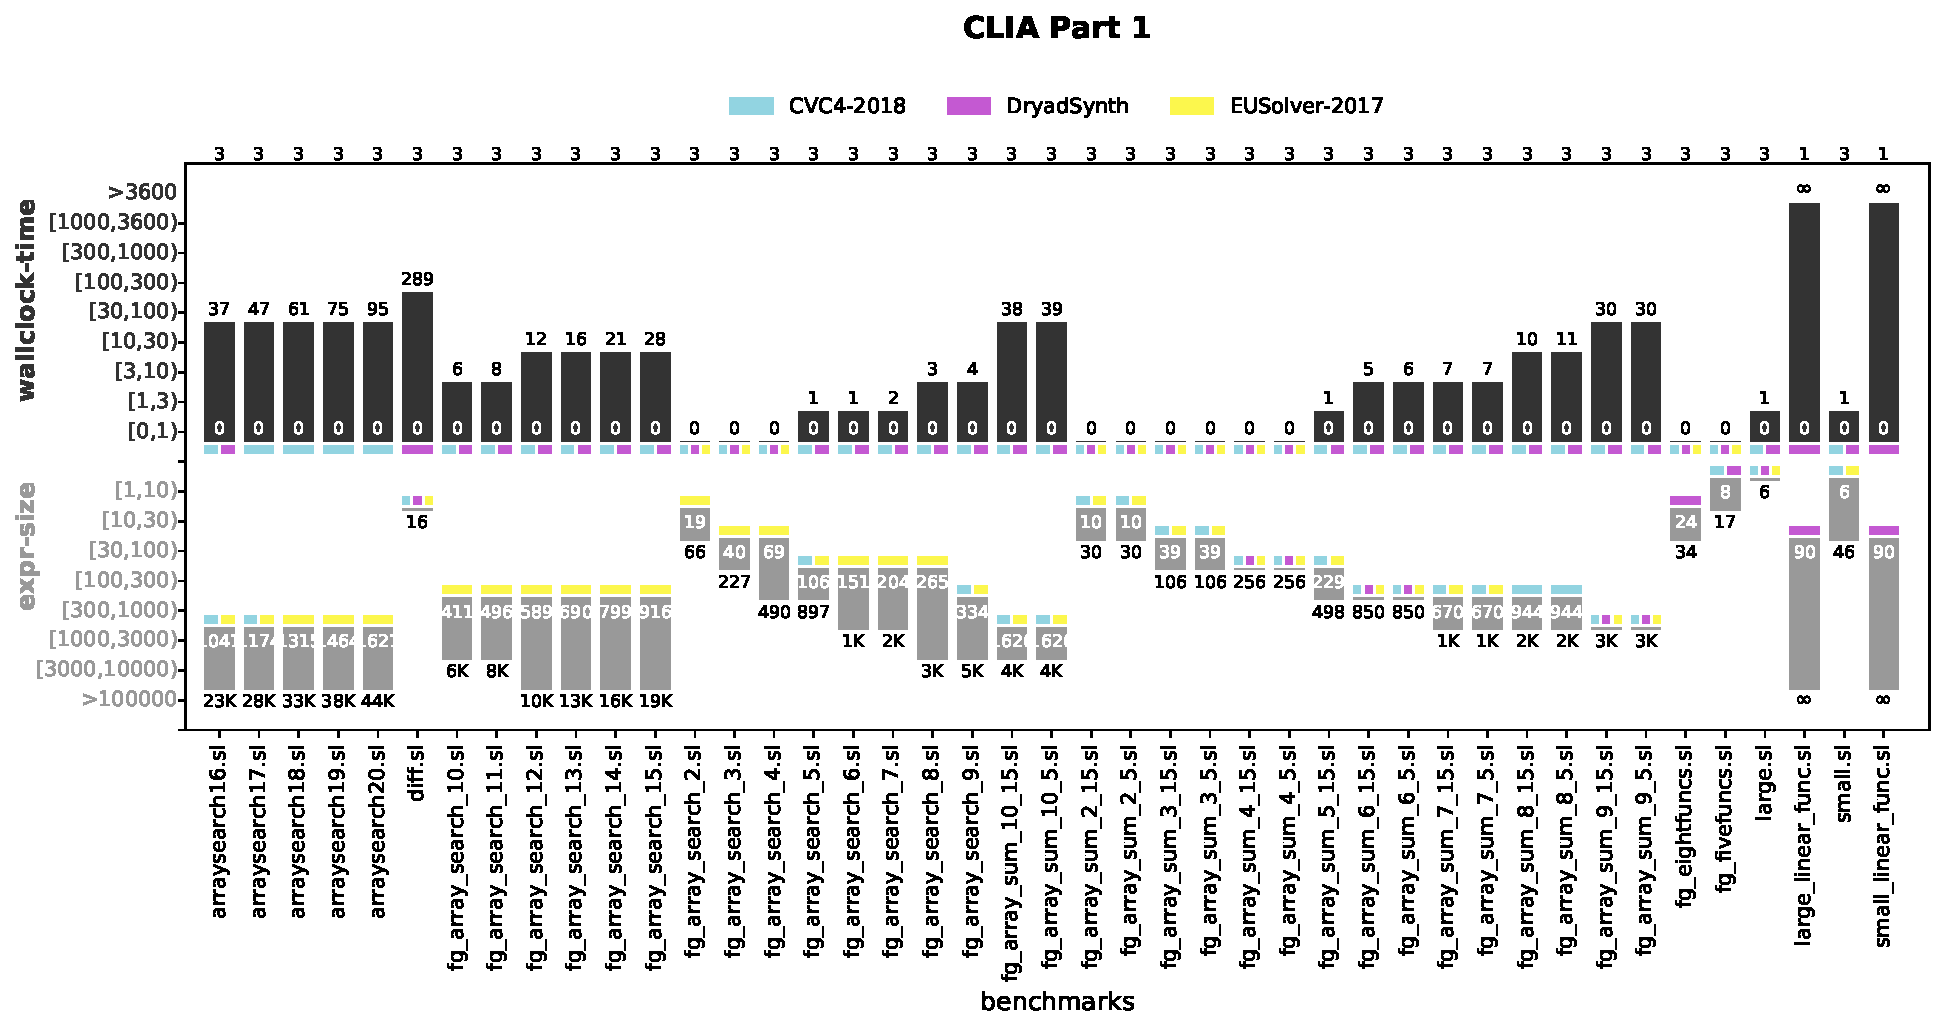
\includegraphics[width=10in]{figures/CLIA1.pdf} \\[3cm]
				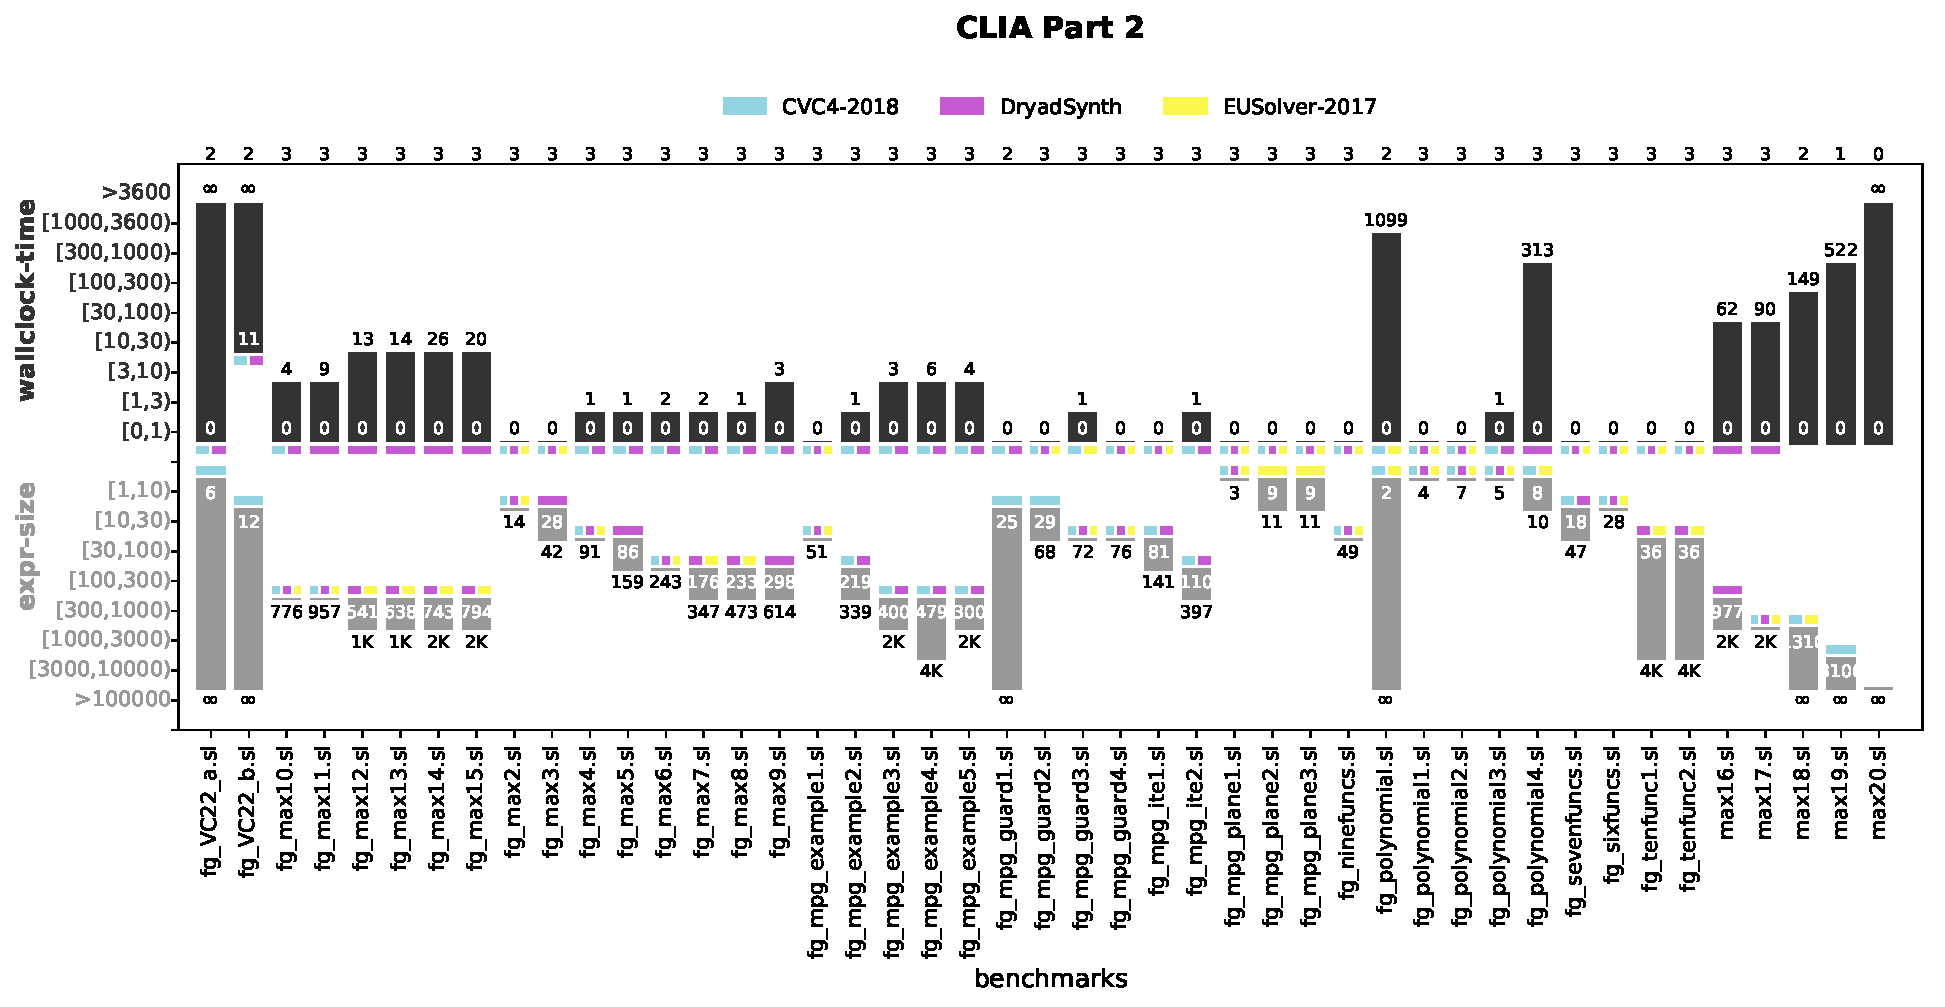
\includegraphics[width=10in]{figures/CLIA2.pdf} 
			\end{tabular}
	}}
	\caption{Evaluation of CLIA track benchmarks.}
	\label{fig:clia-results}
\end{figure*}



\begin{figure*}
	\noindent\makebox[\textwidth]{
		\scalebox{0.6}{
			\begin{tabular}{c}
				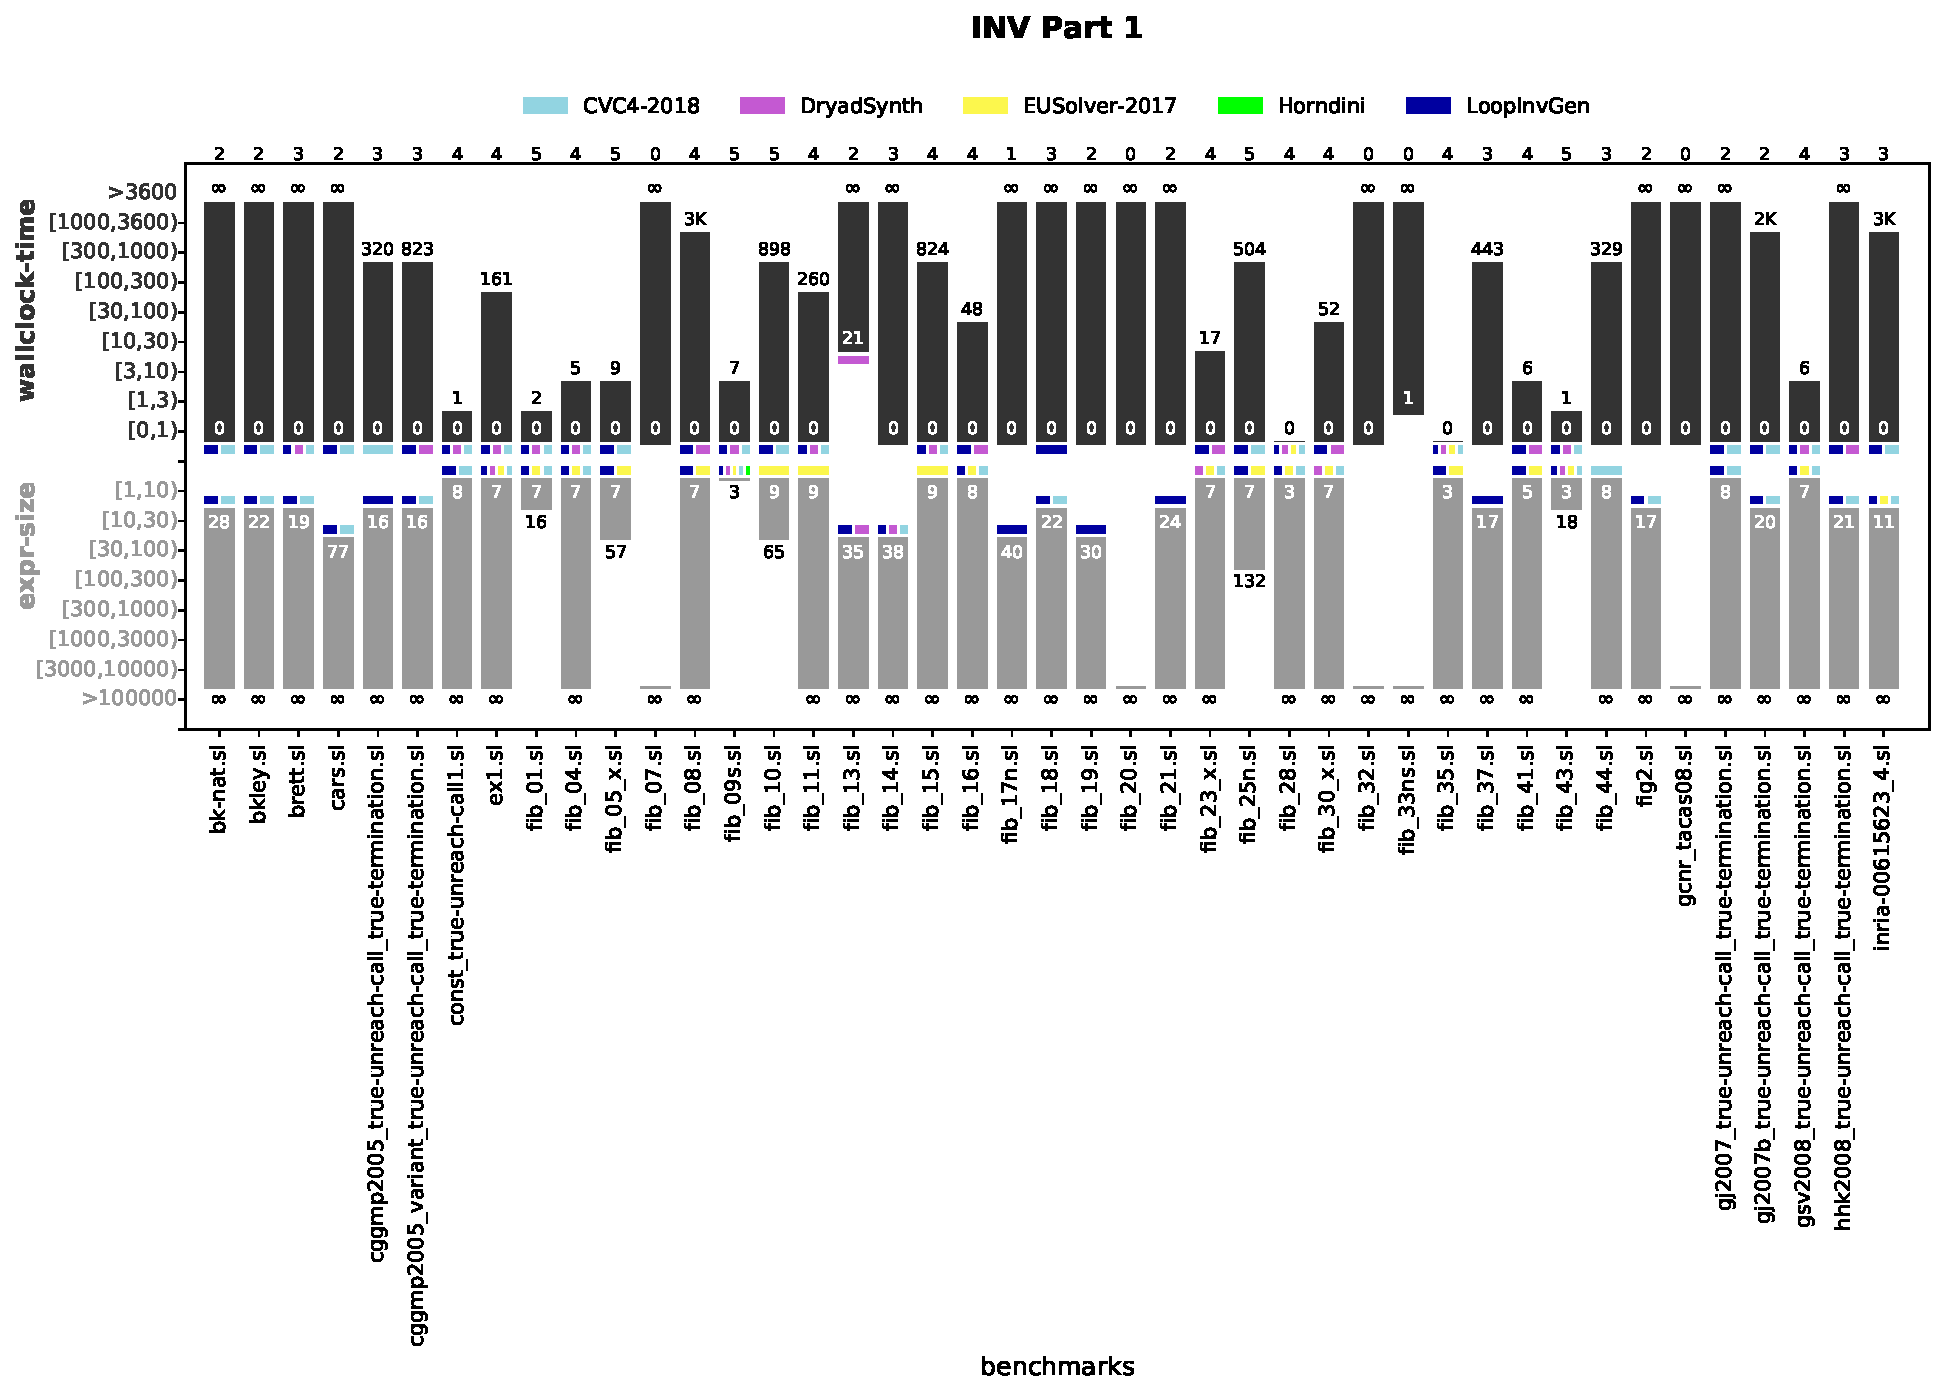
\includegraphics[width=10in]{figures/Inv1.pdf} \\[5mm]
				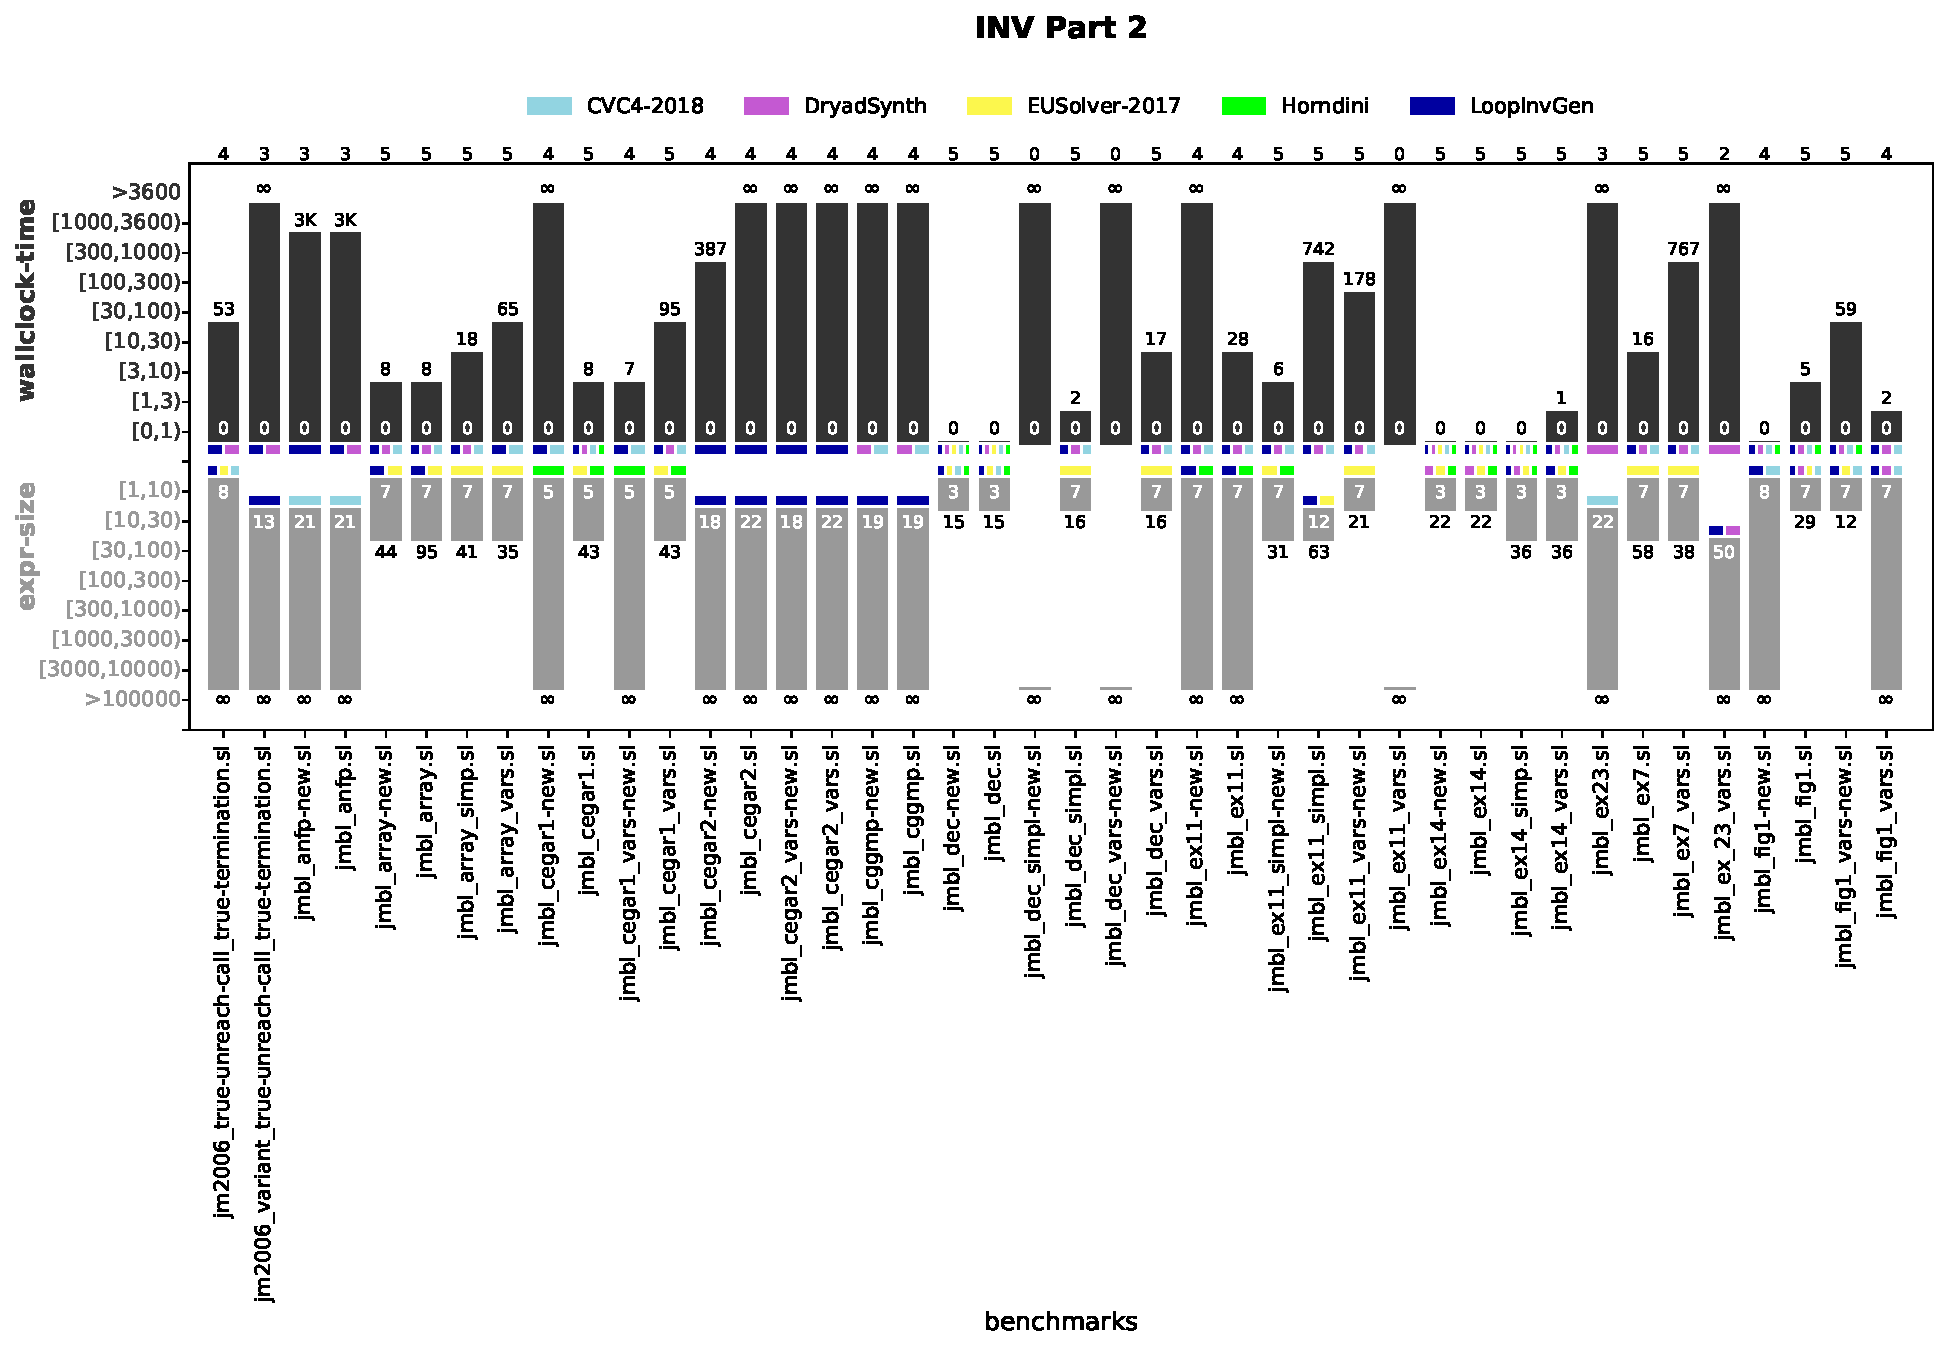
\includegraphics[width=10in]{figures/Inv2.pdf}
			\end{tabular}
	}}
	\caption{Evaluation of Invariant track benchmarks (Parts 1 \& 2).}
	\label{fig:inv-results-1}
\end{figure*}



\begin{figure*}
	\noindent\makebox[\textwidth]{
		\scalebox{0.6}{
			\begin{tabular}{c}
				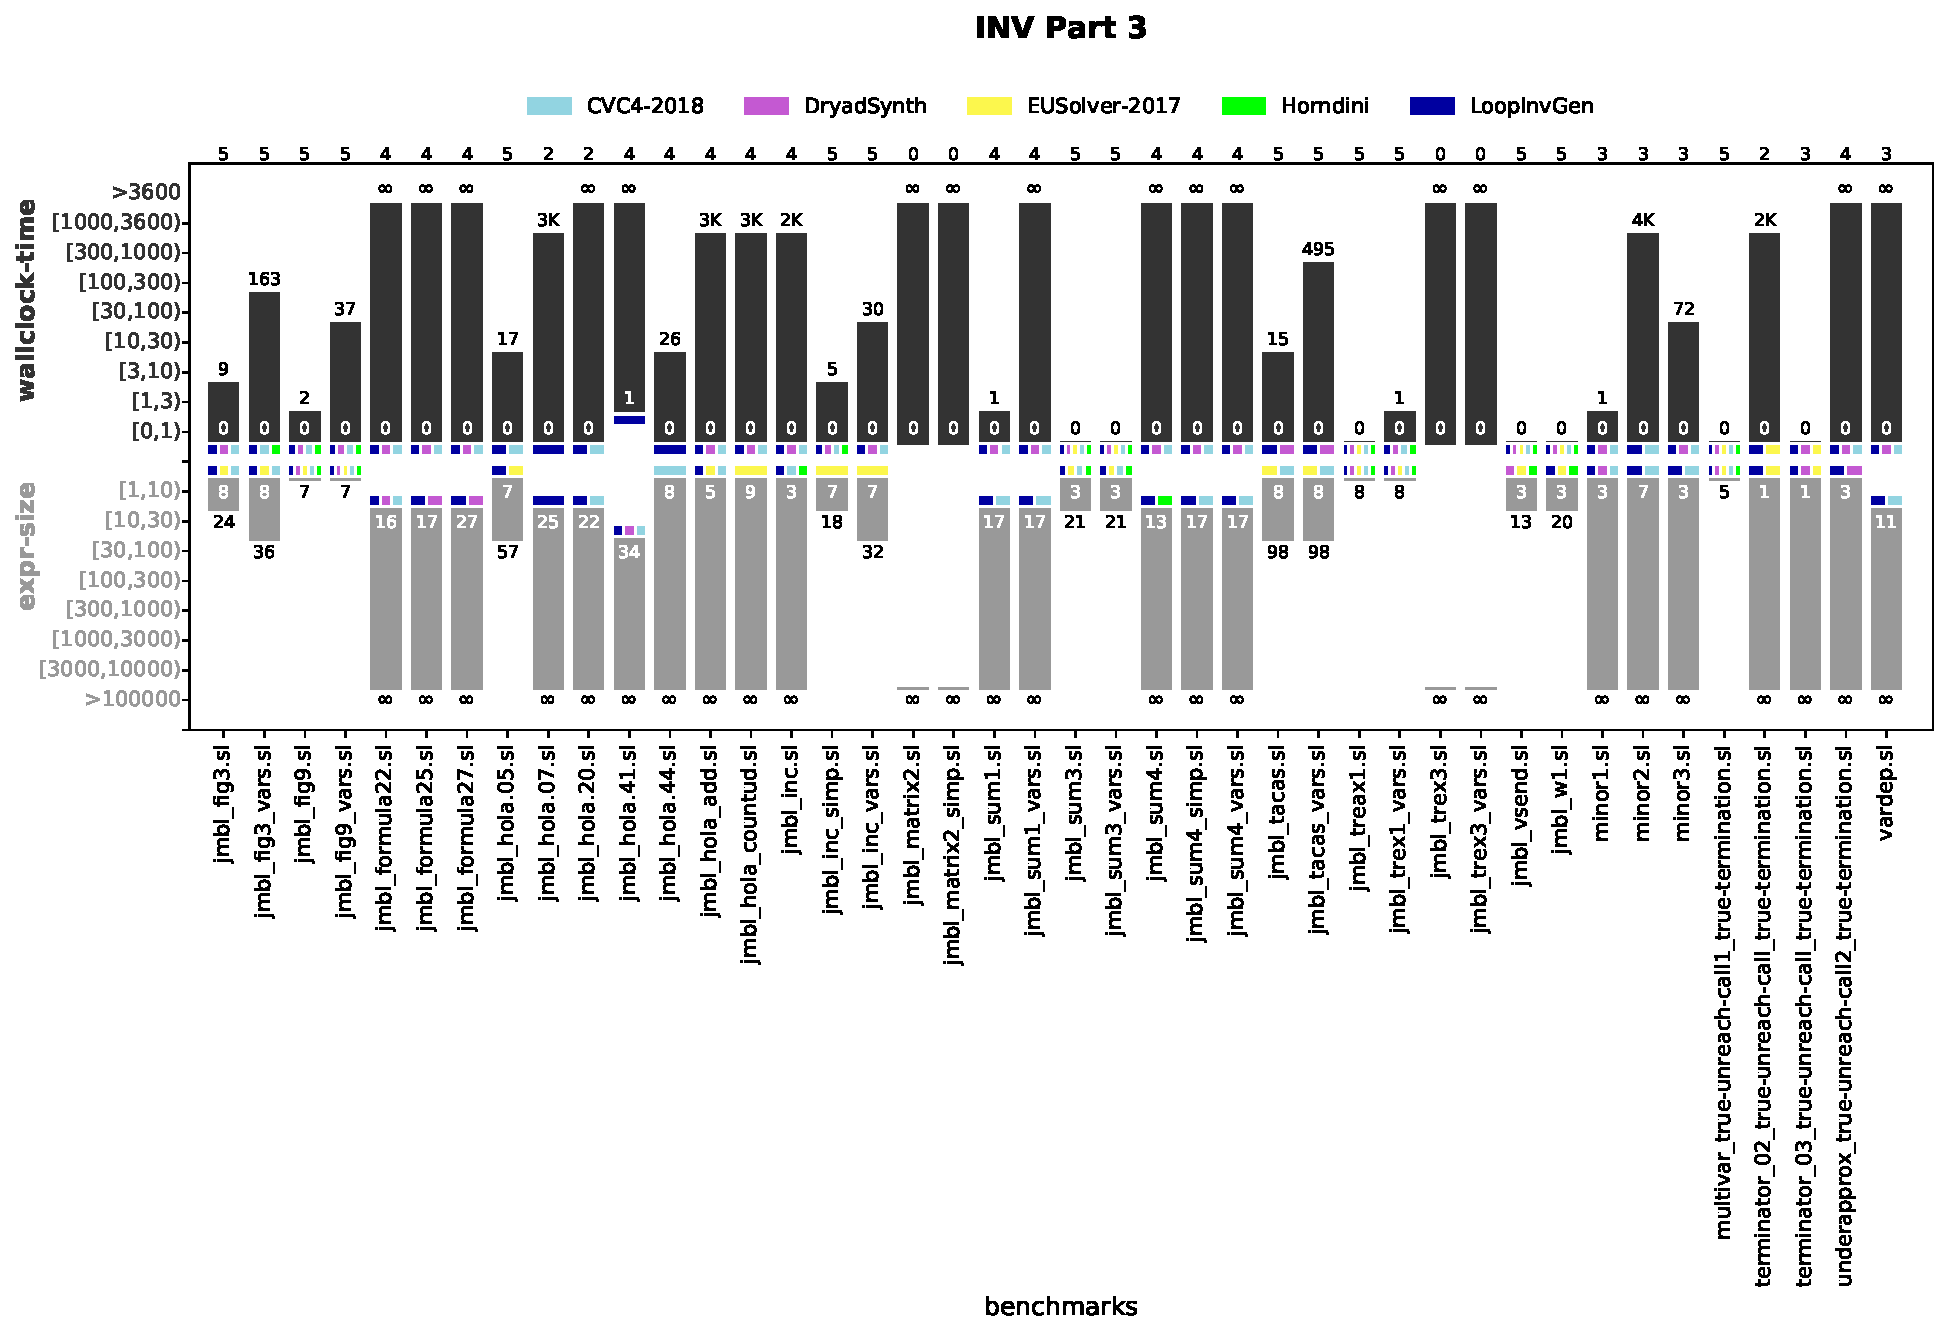
\includegraphics[width=10in]{figures/Inv3.pdf}
			\end{tabular}
		}}
	\caption{Evaluation of Invariant track benchmarks (Part 3).}
	\label{fig:inv-results-2}
\end{figure*}

\begin{figure*}
	\noindent\makebox[\textwidth]{
		\scalebox{0.6}{
			\begin{tabular}{c}
				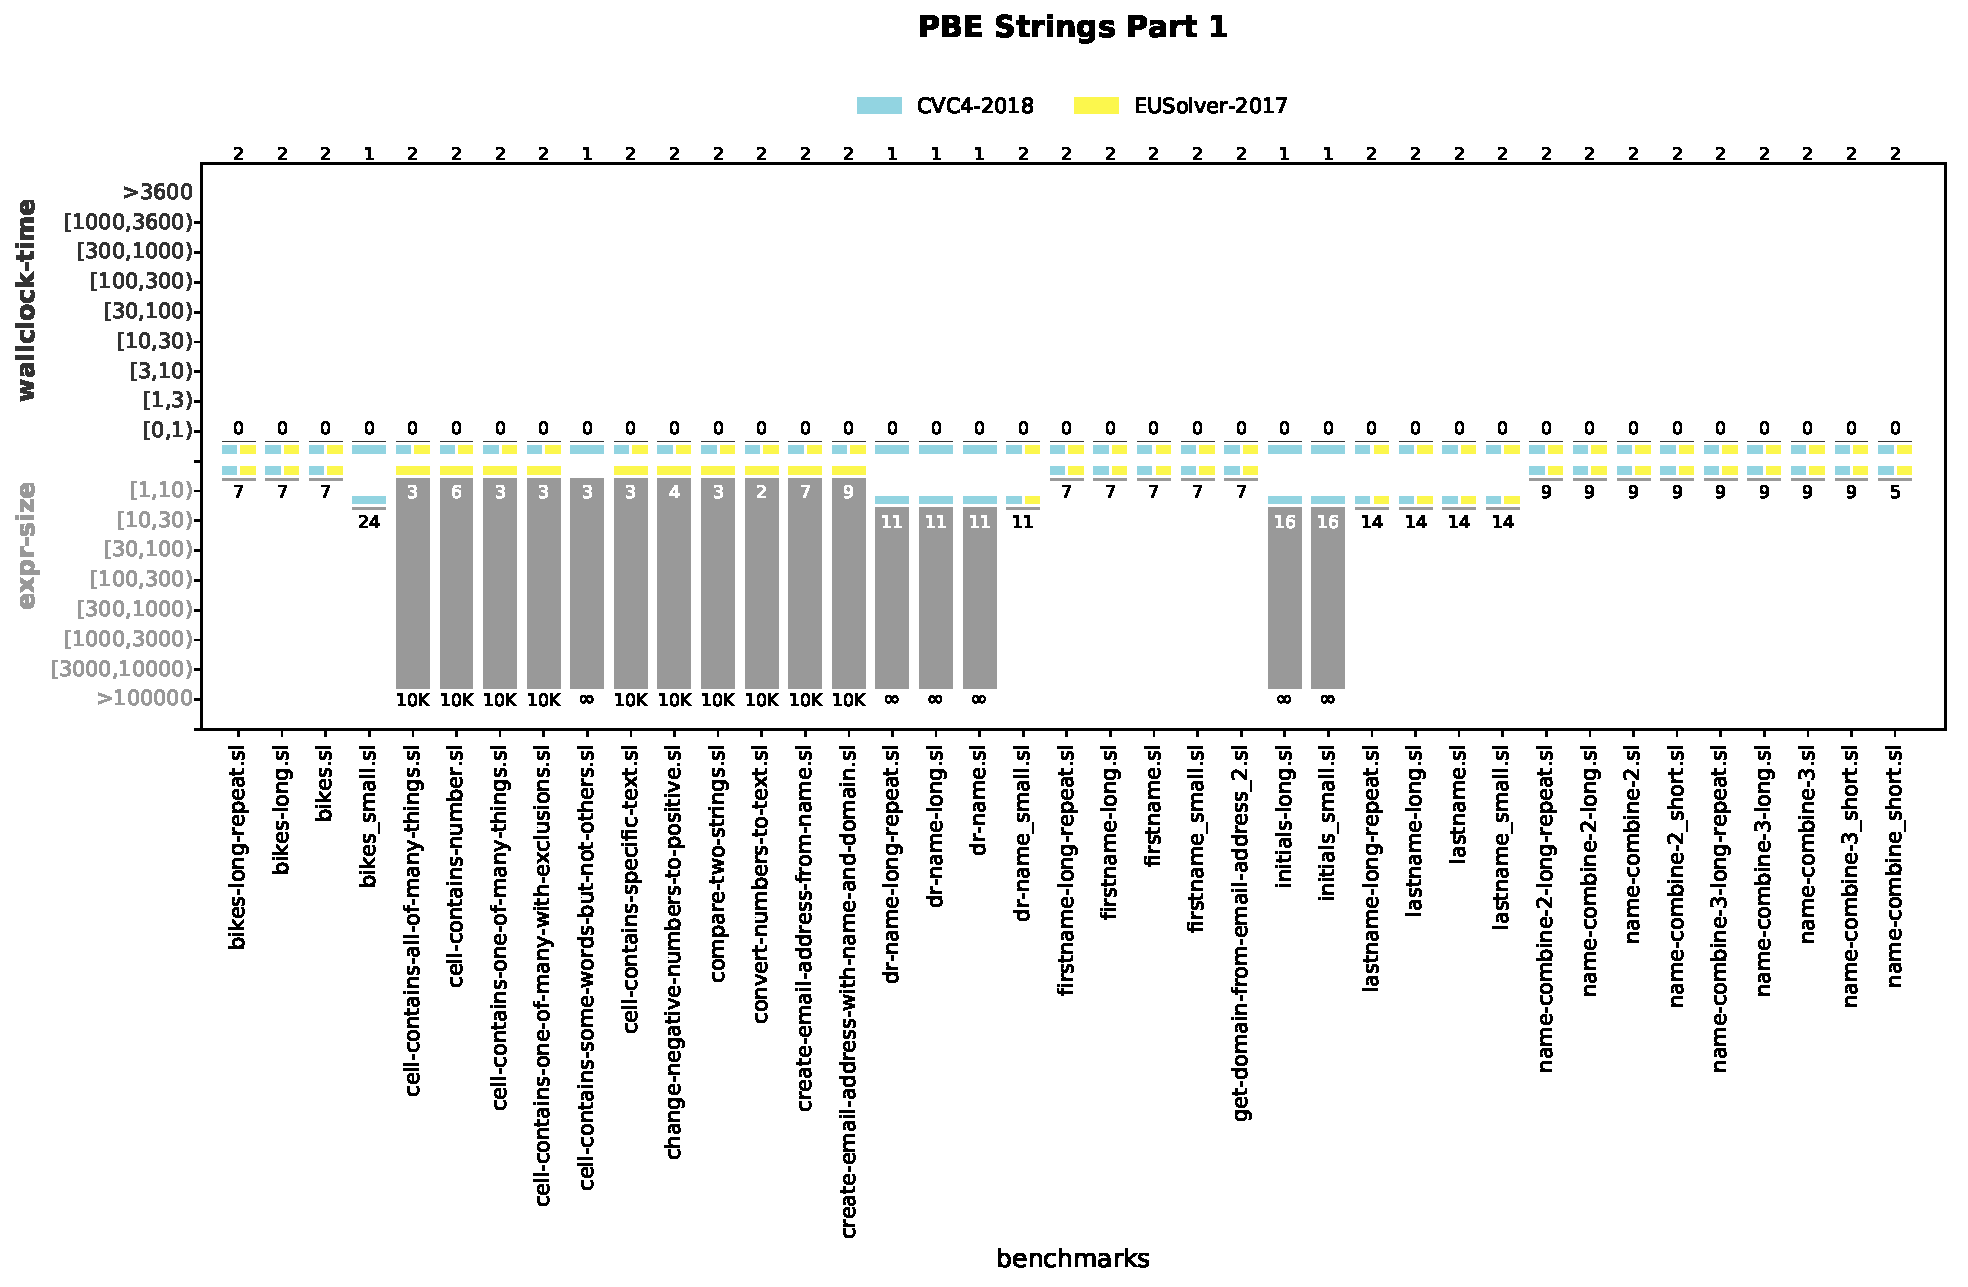
\includegraphics[width=10in]{figures/PBEStrings1.pdf} \\[3cm]
				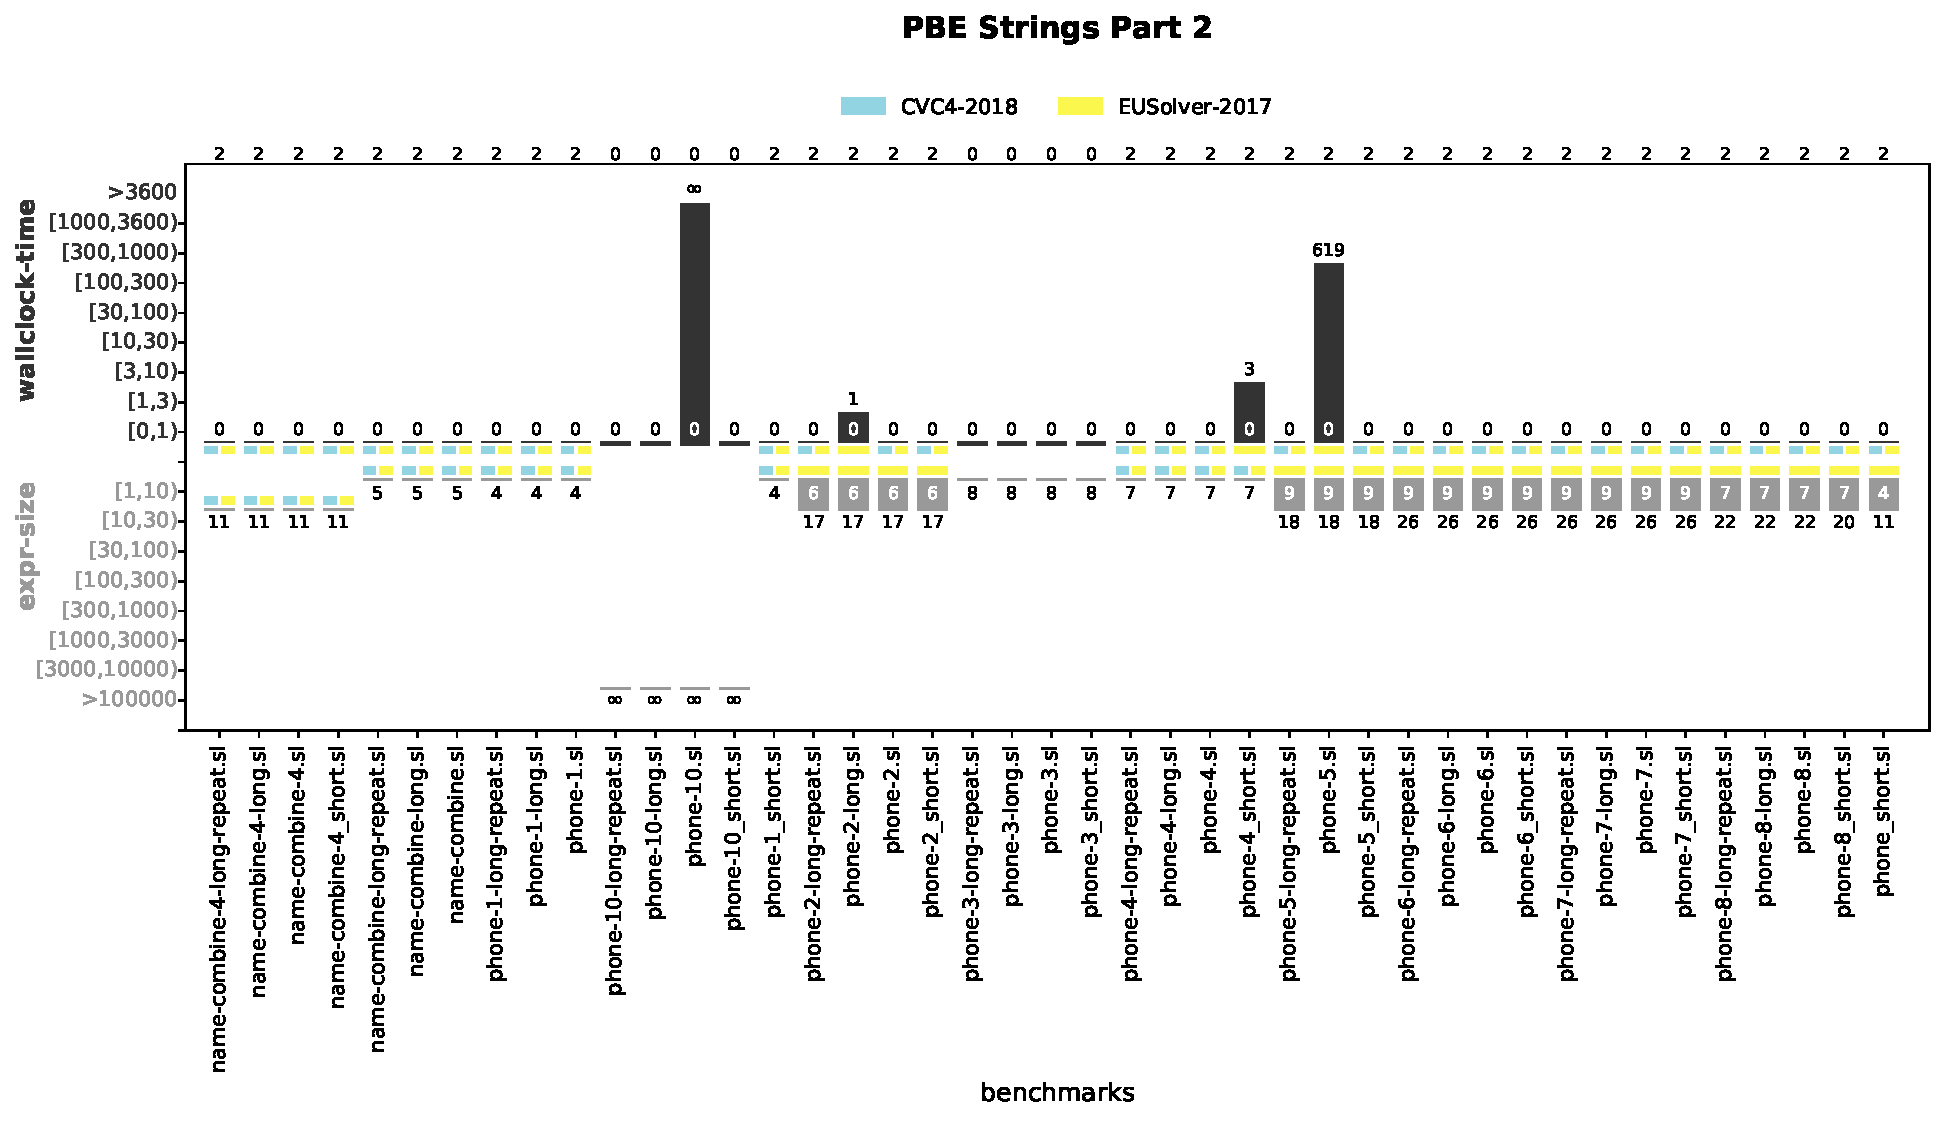
\includegraphics[width=10in]{figures/PBEStrings2.pdf} 
			\end{tabular}
		}}
	\caption{Evaluation of PBE Strings track benchmarks.}
	\label{fig:pbe-strings-results}
\end{figure*}